\documentclass{article}

% if you need to pass options to natbib, use, e.g.:
%     \PassOptionsToPackage{numbers, compress}{natbib}
% before loading neurips_2020

% ready for submission
% \usepackage{neurips_2020}

% to compile a preprint version, e.g., for submission to arXiv, add add the
% [preprint] option:
%     \usepackage[preprint]{neurips_2020}

% to compile a camera-ready version, add the [final] option, e.g.:
%     \usepackage[final]{neurips_2020}

% to avoid loading the natbib package, add option nonatbib:
\usepackage[preprint]{neurips_2020}
\usepackage[utf8]{inputenc} % allow utf-8 input
\usepackage[T1]{fontenc}    % use 8-bit T1 fonts
\usepackage{hyperref}       % hyperlinks
\usepackage{url}            % simple URL typesetting
\usepackage{booktabs}       % professional-quality tables
\usepackage{amsfonts}       % blackboard math symbols
\usepackage{nicefrac}       % compact symbols for 1/2, etc.
\usepackage{microtype}      % microtypography
\usepackage{bbm}
%!TEX root =  autocontgrlp.tex

\usepackage{multicol}
\usepackage{multirow}
\usepackage{dsfont}
\usepackage{tabularx}
%\setlength{\marginparwidth}{13mm}
\usepackage[textsize=tiny]{todonotes}
%\usepackage[disable]{todonotes}
\newcommand{\todoch}[2][]{\todo[color=blue!20!white,#1]{C: #2}}
%\usepackage{enumitem}
%\usepackage[fleqn]{amsmath}
\usepackage{amsmath}
\usepackage{mathtools}
\usepackage{graphicx}
\usepackage{times}
\usepackage{helvet}
\usepackage{courier}
\usepackage{paralist}
\usepackage{latexsym}
\usepackage{url}
\usepackage[all]{xy}
\usepackage{amsmath}
\usepackage{amssymb}
\usepackage{amsthm}
\usepackage{nccmath} % mfrac
\usepackage{comment}
%\usepackage{enumitem}
\usepackage{paralist}
\usepackage{xcolor}
%\usepackage[colorlinks=true,linkcolor=blue,citecolor=purple]{hyperref}
%\usepackage{hyperref}
\usepackage{graphicx}
\usepackage{pifont}
%\usepackage{algorithm}
%\usepackage{algorithmic}
%\usepackage{pseudocode}
%\usepackage{algpseudocode}
\usepackage{savesym}
\savesymbol{AND}
\usepackage{xspace}
\usepackage{tikz}
\usepackage{pgfplots}
\usepackage{pgf}
\usepackage{algorithm}
\usepackage{algorithmic}
\usepackage{xspace}
\usepackage{comment}
\usepackage{placeins}
%\usepackage[capitalize]{cleveref}
%\usepackage{caption}

%\usepackage{style/ssltr}
%\usepackage{style/macros}
\if0
\usetikzlibrary{intersections}
\usetikzlibrary{arrows,calc,fit,patterns,plotmarks,shapes.geometric,shapes.misc,shapes.symbols,   shapes.arrows,   shapes.callouts,   shapes.multipart,   shapes.gates.logic.US,   shapes.gates.logic.IEC,   er,   automata,   backgrounds,   chains,   topaths,   trees,   petri,   mindmap,   matrix,   calendar,   folding, fadings,   through,   positioning,   scopes,   decorations.fractals,   decorations.shapes,   decorations.text,   decorations.pathmorphing,   decorations.pathreplacing,   decorations.footprints,   decorations.markings, shadows,circuits}
\tikzstyle{decision}=[diamond,draw]
\tikzstyle{line}=[draw]
\tikzstyle{elli}=[draw,ellipse]
\tikzstyle{arrow} = [thick]
\fi
%\usepackage{subfig}

\newcommand{\rsa}{\rightsquigarrow}

\newcommand{\mb}{\mbox{ }}
\newcommand{\one}{\mathbf{1}}
\newcommand{\zero}{\mathbf{0}}
\newcommand{\nn}{\nonumber}

\newcommand{\inrdnet}{\in\R^{d_{net}}}
\newcommand{\inrdin}{\in\R^{d_{in}}}
\newcommand{\R}{\Re} %{\mathbb{R}}
\newcommand{\Rm}{\mathbf{R}_{\min}}
\newcommand{\ra}{\rightarrow}
\newcommand{\om}{\otimes}
\newcommand{\op}{\oplus}
\newcommand{\RA}{\Rightarrow}
\newcommand{\LA}{\Leftarrow}
%\newcommand{\E}{\mathbb{E}}
\newcommand{\E}[1]{\mathbb{E}\left[#1\right]}
\newcommand{\lmin}[1]{\lambda_{\min}\left(#1\right)}
\newcommand{\T}{\mathcal{T}}
\newcommand{\B}{\mathcal{B}}
\newcommand{\F}{\mathcal{F}}
\newcommand{\C}{\mathcal{C}}
\newcommand{\M}{\mathcal{M}}
\newcommand{\N}{\mathcal{N}}
\newcommand{\V}{\mathcal{V}}
\newcommand{\I}{\mathcal{I}}

\newcommand{\mm}{m_{-}}
\newcommand{\mdm}{m'_{-}}
\newcommand{\Tvm}{\Theta^{v,\mm}}
\newcommand{\Tvmd}{\Theta^{v,\mdm}}

\newcommand{\psiv}{\psi^{\text{V}}}
\newcommand{\psif}{\psi^{\text{F}}}

\newcommand{\kv}{K^{\text{V}}_{\Theta}}
\newcommand{\kf}{K^{\text{F}}_{\Theta}}
\newcommand{\kc}{K^{\text{CROSS}}_{\Theta}}

%\newcommand{\Tb}{\mathbf{\Theta}}
%\newcommand{\Tv}{\mathbf{\Theta}^v}
%\newcommand{\Tw}{\mathbf{\Theta}^w}
\newcommand{\tv}{{\theta^{\text{V}}}}

\newcommand{\Tdgn}{\Theta^{\text{DGN}}}
\newcommand{\Tb}{{\Theta}}
\newcommand{\Tv}{{\Theta}^{\text{V}}}
%\newcommand{\Tw}{{\Theta}^w}
\newcommand{\Tg}{{\Theta}^{\text{F}}}

\newcommand{\tg}{\theta^{\text{F}}}
%\newcommand{\Tg}{\mathbf{\Theta}^g}
\newcommand{\Tt}{\Theta}

\newcommand{\G}{\mathcal{G}}

\DeclareMathOperator{\argmin}{argmin}
\DeclareMathOperator{\argmax}{argmax}
\newcommand{\norm}[1]{\|#1\|}
\newcommand{\inorm}[1]{\|#1\|_{\infty}}
\newcommand{\snorm}[1]{\left\|#1\right\|}
\newcommand{\sinorm}[1]{\left\|#1\right\|_{\infty}}


%\newcommand{\eqdef}{\stackrel{\text{\footnotesize def}}{=}}
%\newcommand{\eqdef}{\stackrel{\Delta}{=}}
\newcommand{\eqdef}{\doteq}
\newcommand{\defeq}{\doteq}

\newcommand{\eps}{\varepsilon}
\renewcommand{\epsilon}{\varepsilon}

\newcommand{\nt}{\nabla_{\Theta}}
\newcommand{\al}{\mathcal{AL}}
\newcommand{\aw}{\mathcal{AW}}
\newcommand{\ap}{\mathcal{AP}}

\newcommand{\keywords}[1]{{\bf Keywords: } #1\par}
%\newenvironment{proof}{{\bf Proof:} }{}
\newtheorem{theorem}{Theorem}[section]
\newtheorem{lemma}{Lemma}[section]
\newtheorem{claim}[theorem]{Claim}
\newtheorem{proposition}{Proposition}[section]
\newtheorem{corollary}[theorem]{Corollary}
\newtheorem{assumption}{Assumption}[section]
\newtheorem{definition}{Definition}[section]
\newtheorem{remark}{Remark}[section]
\newtheorem{identity}{Identity}[section]
\newtheorem{example}{Example}[section]
\newtheorem{note}{Note}[section]
\newtheorem{notation}{Notation}[section]
\newcommand{\alert}[1]{\textcolor{red}{#1}} 
\newcommand{\J}{\mathcal{J}}
\newcommand{\ip}[1]{\langle #1\rangle}

\def\v{\mathbf{v}}
\def\r{\mathbf{r}}
\def\p{\mathbf{p}}
\def\q{\mathbf{q}}
%\def\R{\mathrm{R}}
\def\Re{\mathbb{R}}
\def\Z{\mathbb{Z}}
\def\P{\mathcal{P}}
\def\S{\mathcal{S}}
\def\A{\mathcal{A}}
\def\X{\mathcal{X}}
\def\U{\mathcal{U}}

%\newcommand{\B}{\mathcal{B}}


\newcommand{\ith}[2][th]{$#2^{\text{#1}}$}
\newcommand{\us}[2]{\underset{#2}{#1}~}
\newcounter{subequation}[equation]
\newcommand{\thesubequationonly}{\alph{subequation}}
\renewcommand{\thesubequation}{\text{\theequation(\thesubequationonly)}}
\newcommand{\subequationitem}{\refstepcounter{subequation}(\thesubequationonly)\thinspace}

\def\mathdisplay#1{%
  \ifmmode \@badmath
  \else
    $\def\@currenvir{#1}%
    \let\dspbrk@context\z@
    \let\tag\tag@in@display \SK@equationtrue %\let\label\label@in@display
    \global\let\df@label\@empty \global\let\df@tag\@empty
    \global\tag@false
    \let\mathdisplay@push\mathdisplay@@push
    \let\mathdisplay@pop\mathdisplay@@pop
    \if@fleqn
      \edef\restore@hfuzz{\hfuzz\the\hfuzz\relax}%
      \hfuzz\maxdimen
      \setbox\z@\hbox to\displaywidth\bgroup
        \let\split@warning\relax \restore@hfuzz
        \everymath\@emptytoks \m@th $\displaystyle
    \fi
%   \fi
}

\newcommand{\algorithmicinput}{\textbf{Input:} }
\newcommand{\INPUT}{\item[\algorithmicinput]}
\newcommand{\algorithmicoutput}{\textbf{Output:} }
\newcommand{\OUTPUT}{\item[\algorithmicoutput]}
\newcounter{algostep}
\newcommand{\Step}[1][\STATE]{#1\textbf{\refstepcounter{algostep}\thealgostep}. }

\newenvironment{algoequation}{\refstepcounter{equation}$}{$\hfill (\theequation)}

\newenvironment{nonfloatalgorithm}[1]{\vspace{1ex}\hrule\vspace{0.5ex} \refstepcounter{algorithm}\textbf{Algorithm \thealgorithm}\hspace{1em} #1 \vspace{0.5ex}\hrule}{\hrule\vspace{1.5ex}\setcounter{algostep}{0}}

\newcounter{acalgorithm}

\newenvironment{nonfloatactorcriticalgorithm}[1]{\vspace{1ex}\hrule\vspace{0.5ex} \textbf{Actor-Critic Algorithm \refstepcounter{acalgorithm}\theacalgorithm}\hspace{1em} #1 \vspace{0.5ex}\hrule\addcontentsline{loa}{algorithm}{\protect\numberline{\theacalgorithm}{\ignorespaces #1}}}{\hrule\vspace{1.5ex}\setcounter{algostep}{0}}

\usepackage{hyperref}
\usepackage{thmtools}
\usepackage{nameref}

\usepackage[nameinlink,noabbrev,capitalize]{cleveref}
\crefname{assumption}{assumption}{assumptions}
\crefname{lemma}{lemma}{lemmas}
\Crefname{lemma}{Lemma}{Lemmas}
\crefname{thm}{theorem}{theorems}
\Crefname{thm}{Theorem}{Theorems}
\crefname{proposition}{proposition}{propositions}



\usepackage{caption}
\captionsetup{belowskip=0pt}
\usepackage{wrapfig,lipsum}
\usepackage[linewidth=1.2pt,linecolor=red]{mdframed}


\usepackage{comment}
\usepackage{cancel}
\usepackage{changepage}
\usepackage{bbm}
\usepackage{pgfplots}
\usepackage{filecontents}
\setcounter{MaxMatrixCols}{32}
\usepackage{placeins}

\title{Neural Path Features and Neural Path Kernel : Understanding the role of gates in deep learning}
% The \author macro works with any number of authors. There are two commands
% used to separate the names and addresses of multiple authors: \And and \AND.
%
% Using \And between authors leaves it to LaTeX to determine where to break the
% lines. Using \AND forces a line break at that point. So, if LaTeX puts 3 of 4
% authors names on the first line, and the last on the second line, try using
% \AND instead of \And before the third author name.
\author{Chandrashekar Lakshminarayanan${}^*$ and Amit Vikram Singh\thanks{Both authors contributed equally.},\\ Indian Institute of Technology Palakkad\\\{chandru@iitpkd.ac.in,amitkvikram@gmail.com\}}
\begin{document}
\maketitle
\begin{abstract}
Rectified linear unit (ReLU) activations can also be thought of as \emph{gates}, which, either pass or stop their pre-activation input when they are \emph{on} (when the pre-activation input is positive) or \emph{off} (when the pre-activation input is negative) respectively. A deep neural network (DNN) with ReLU activations has many gates, and the {on/off} status of each gate changes across input examples as well as network weights. For a given input example, only a subset of gates are \emph{active}, i.e., on, and the sub-network of weights connected to these active gates is responsible for producing the output. At randomised initialisation, the active sub-network corresponding to a given input example is random. During training, as the weights are learnt,  the active sub-networks are also learnt, and potentially hold very valuable information. 

In this paper, we analytically characterise the role of active sub-networks in deep learning. To this end, we encode the {on/off} state of the gates of a given input in a novel \emph{neural path feature} (NPF), and the weights of the DNN are encoded in a novel \emph{neural path value} (NPV). Further, we show that the output of network is indeed the inner product of NPF and NPV.  The main result of the paper shows that the \emph{neural path kernel} associated with the NPF is a fundamental quantity that characterises the information stored in the gates of a DNN. We show via experiments (on MNIST and CIFAR-10) that in standard DNNs with ReLU activations NPFs are learnt during training and such learning is key for generalisation. Furthermore, NPFs and NPVs can be learnt in two separate networks and such learning also generalises well in experiments. In our experiments, we observe that almost all the information learnt by a DNN with ReLU activations is stored in the gates - a novel observation that underscores the need to further investigate the role of gating in DNNs.
\end{abstract}

\section{Introduction}
We consider deep neural networks (DNNs) with rectified linear unit (ReLU) activations. A special property of ReLU activation is that it can be written as a product of its pre-activation input, say $q\in\R$ and a gating signal, $\gamma_r(q)=\mathbbm{1}_{\{q>0\}}$, i.e., $\chi_r(q)=q\cdot\gamma_r(q)$. In what follows, we call $\chi_r$ as the ReLU activation and $\gamma_r$ as the ReLU gate.  While the weights (of a DNN) remain the same across input examples, the $1/0$ state of the gates (or simply gates) change across input examples. For each input example, there is a corresponding \emph{active} sub-network consisting of those gates which are $1$, and the weights which pass through such gates. This active sub-network can be said to hold the memory for a given input, i.e., only those weights that pass through such active gates contribute to the output. In this viewpoint, at random initialisation of the weights, for a given input example, a random sub-network is active and produces a random output.  However, as the weights change during training (say via gradient descent), the gates change, and hence the active sub-networks corresponding to the various input examples also change. At the end of training, for each input example, there is a learned active sub-network, and produces a learned output. Thus, the gates of a trained DNN could potentially contain valuable information. In this paper, we study the role of the gates, and the dynamics of the gates while training DNNs  using gradient descent (GD). Our findings can be summarised in the following claims which we theoretically/experimentally justify in the paper:

Claim I  (see \Cref{sec:infomeasure}): \emph{Active sub-networks are fundamental entities in DNNs with ReLU activations.}  

Claim II (see \Cref{sec:experiments}): \emph{Learning of the active sub-networks during training is key for generalisation.}

Before we discuss ``Claims I and II'' in terms of our novel contributions in \Cref{sec:contrib}, we present the background of  \emph{neural tangent feature and kernel} (NTF and NTK) in \Cref{sec:background}.

\textbf{Notation:} We denote the set $\{1,\ldots, n\}$ by $[n]$. For $x,y\in\R^m$, $\ip{x,y}=x^\top y$. The maximum and minimum eigenvalue of a real symmetric matrix $A$ are denoted by $\rho_{\max}(A)$ and $\rho_{\min}(A)$. We consider fully-connected DNNs with $w$ hidden units per layer and $d-1$ hidden layers. The output of the DNN for an input $x\in\R^{d_{in}}$ is denoted by $\hat{y}_{\Theta}(x)\in\R$, where $\Theta\inrdnet$ are the network weight ($d_{net}=d_{in}w+(d-2)w^2+w$). We denote by $\Theta(l,j,i)$, the weight connecting the $j^{th}$ hidden unit of layer $l-1$ to the $i^{th}$ hidden unit of layer $l\in[d]$. $\Theta(1)\in\R^{w\times d_{in}}, \Theta(l)\in\R^{w\times w},\forall l\in\{2,\ldots,d-1\}, \Theta(d)\in\R^{w\times 1}$. The dataset is given by $(x_s,y_s)_{s=1}^n\in\R^{d_{in}}\times \R$. The loss function is given by $L_{\Theta}=\frac{1}{2}\sum_{s=1}^n \left(\hat{y}_{\Theta}(x_s)-y_s\right)^2$. We use $\nabla_{\Theta}(\cdot)$ stands for the gradient of $(\cdot)$ with respect to the network weights. We use vectorised notations $y=(y_s,s\in[n]), \hat{y}_{\Theta}=\left(\hat{y}_{\Theta}(x_s), s\in[n]\right)\in\R^n$ for the true and predicted outputs and $e_{t}= (\hat{y}_{\Theta_t}-y)\in\R^n$ for the error in the prediction. We use $\theta\in\Theta$ to denote single arbitrary weight, and $\partial_{\theta}(\cdot)$ to denote $\frac{\partial (\cdot)}{\partial \theta}$.  $\Sigma\in\R^{n\times n}$ is the input Gram matrix with entries $\Sigma(s,s')=\ip{x_s,x_{s'}}$.
%We consider the gradient descent update given by $\Theta_t=\Theta_t-\alpha_t (\nabla_{\Theta} L_{\Theta_t})$, where $\alpha_t>0$ is a small step-size and 
\subsection{Background: Neural Tangent Feature and Kernel}\label{sec:background}
The NTF and NTK machinery was developed in some of the recent works [\citenum{ntk, arora2019exact,cao2019generalization,dudnn}] to understand optimisation and generalisation in DNNs trained using GD. For an input $x\in\R^{d_{in}}$, the NTF is given by $\psi_{x,\Theta}=\nabla_{\Theta}\hat{y}_{\Theta}(x)\inrdnet$, i.e.,  the gradient of the network output with respect to its weights. The NTK matrix $K_{\Theta}$ on the dataset is the $n\times n$ Gram matrix of the NTFs of the input examples, and is given by $K_{\Theta}(s,s')=\ip{\psi_{x_s,\Theta},\psi_{x_{s'},\Theta}}, s,s'\in[n]$. 
\begin{proposition}[\textbf{Lemma 3.1} \cite{arora2019exact}]\label{prop:basic}
Consider the GD procedure to minimise the  squared loss $L(\Theta)$ with infinitesimally small step-size: $\dot{\Theta}_t=-\nabla_{\Theta}L_{\Theta_t} $. If follows that the dynamics of the error term can be written as $\dot{e}_t=-K_{\Theta_t} e_t$. 
\end{proposition}

\textbf{Prior works} [\citenum{ntk,dudnn,arora2019exact,cao2019generalization}] have studied DNNs trained using GD in the so called `NTK regime', which occurs under appropriate randomised initialisation, and when the width of the DNN approaches infinity. The characterising property of the NTK regime is that as $w\ra\infty$, $K_{\Theta_0}\ra K^{(d)}$, and $K_{\Theta_t}\approx K_{\Theta_0}$, where $K^{(d)}$ (see \eqref{eq:ntkold} in \Cref{sec:kd}) is a deterministic matrix whose superscript $(d)$ denotes the depth of the DNN. 
\begin{comment}
The $K^{(d)}$ matrix is computed by the recursion in \eqref{eq:ntkold}.
\begin{align}\label{eq:ntkold}
&\tilde{K}^{(1)}(s,s')=\Sigma^{(1)}(s,s')=\Sigma(s,s'), M^{(l)}_{ss'}=\left[\begin{matrix}\Sigma^{(l)}(s,s) & \Sigma^{(l)}(s,s')\\ \Sigma^{(l)}(s',s) & \Sigma^{(l)}(s',s')\end{matrix}\right]\in \R^2,\\
&\Sigma^{(l+1)}(s,s')= 2\cdot\mathbb{E}_{(q,q')\sim N(0,M_{ss'}^{(l)})} \left[\chi(q)\chi(q')\right], \hat{\Sigma}^{(l+1)}(s,s')= 2\cdot\mathbb{E}_{(q,q')\sim N(0,M_{ss'}^{(l)})}\left[\partial\chi(q)\partial{\chi}(q')\right],\nn\\
&\tilde{K}^{(l+1)}=\tilde{K}^{(l)}\odot \hat{\Sigma}^{(l+1)}+\Sigma^{(l+1)}, K^{(d)}=\left(\tilde{K}^{(d)}+\Sigma^{(d)}\right)/2
\end{align}
where $s,s'\in[n]$ are two input examples in the dataset, $\Sigma$ is the data Gram matrix, $\partial{\chi}$ stands for the derivative of the activation function with respect to the pre-activation input, $N(0,M)$ stands for the mean-zero Gaussian distribution with co-variance matrix $M$.
\end{comment}
\cite{arora2019exact} show that infinite width DNN trained using GD is equivalent to kernel regression with the limiting NTK matrix $K^{(d)}$ (and hence enjoys the generalisation ability of the limiting NTK matrix $K^{(d)}$). Further, \cite{arora2019exact} propose a pure kernel method based on what they call the CNTK, which is the limiting NTK matrix $K^{(d)}$ for an infinite width convolutional neural network (CNN). \cite{cao2019generalization} show that in the NTK regime, a DNN is almost a linear learner with the random NTFs at initialisation, and show a generalisation bound in the form of $\tilde{\mathcal{O}}\left(d\cdot\sqrt{y^\top {\left(K^{(d)}\right)}^{-1} y/n}\right)$\footnote{$a_t=\mathcal{O}(b_t)$ if $\lim\sup_{t\ra\infty}|a_t/b_t|<\infty$, and $\tilde{\mathcal{O}}(\cdot)$ is used to hide logarithmic factors in $\mathcal{O}(\cdot)$.}. 

\textbf{Open Question:} \cite{arora2019exact} report a $5\% - 6\%$ performance gain of finite width CNNs (which do not operate in the NTK regime) over the exact CNTKs corresponding to infinite width CNNs, and infer that the study of DNNs in the NTK regime cannot fully explain the success of practical neural networks yet. Can we explain the reason for the performance gain of CNNs over CNTK?%Based on this performance gap they infer that finite width is beneficial and and that the study of DNNs in the NTK regime cannot fully explain the success of practical neural networks yet. Can we explain the reason for the performance gain of CNNs over CNTK?

\begin{comment}
Fourth, we find that there is still a $5\% - 6\%$ performance gap between CNTKs and CNNs. Since CNTKs exactly correspond to infinitely wide CNNs, this performance gap implies that finite width has its benefits. Therefore, it is likely that recent theoretical work on over-parameterization that operates in the NTK regime cannot fully explain the success of neural networks yet, and we believe it is an interesting open problem to characterize this gap.
\end{comment}
\subsection{Our Contributions}\label{sec:contrib}
To the best of our knowledge, we are the first to analytically characterise the role played by active sub-networks in deep learning as presented in the `Claims I and II'.  The key contributions can be arranged into three landmarks as described below.

$\bullet$ The first step involves breaking a DNN into individual paths, and each path again into gates and weights.  To this end, we encode the states of the gates in a novel \emph{neural path feature} (NPF) and the weights in a novel \emph{neural path value} (NPV) and express the output of the DNN as an inner product of NPF and NPV (see \Cref{sec:path}). In contrast to NTF/NTK which are \emph{first-order} quantities (based on derivatives with respect to the weights), NPF and NPV are \emph{zeroth-order} quantities. The kernel matrix associated to the NPFs namely the \emph{neural path kernel} (NPK) matrix $H_{\Theta}\in\R^{n\times n}$ has a special structure, i.e., it can be written as a \emph{Hadamard} product of the input Gram matrix, and a correlation matrix $\Lambda_{\Theta}\in\R^{n\times n}$, whose entries $\Lambda_{\Theta}(s,s')$ is equal to the total number of path in the sub-network that is active for both input examples $s,s'\in[n]$. With the $\Lambda_{\Theta}$ matrix we reach our first landmark.
%$H_{\Theta}=\Sigma\odot\Lambda_{\Theta}$, where $\odot$ is the \emph{Hadamard} product, $\Sigma\in\R^{n\times n}$ is the input Gram matrix and $\Lambda_{\Theta}\in\R^{n\times n}$ is a correlation matrix, whose entries $\Lambda_{\Theta}(s,s')$ is equal to the total number of path in the sub-network that is active for both input examples $s,s'\in[n]$. With the $\Lambda_{\Theta}$ matrix we reach our first landmark.%To the best of our knowledge quantities NPF, NPV, NPK and $\Lambda$ are novel and have not appeared in prior work. These novels quantities help us to analytically establish the fact that the active sub-networks play a critical role in deep learning, a fact which was not established analytically in prior works.

$\bullet$  Second step is to characterise performance of active sub-networks in a `stand alone' manner. To this end, we consider a new idealised setting namely fixed NPF (FNPF) setting, wherein, the NPFs are fixed (i.e., held constant) and only the NPV is learnt via gradient descent. In this setting, we show that (see \Cref{th:main}), in the limit of infinite width and under randomised initialisation the NTK converges to a matrix $K^{(d)}_{\text{FNPF}}=\text{constant} \times H_{\text{FNPF}}$, where $H_{\text{FNPF}}\in\R^{n\times n}$ is the NPK matrix corresponding to the fixed NPFs. $K^{(d)}$ matrix of \cite{ntk,arora2019exact,cao2019generalization} becomes the $K^{(d)}_{\text{FNPF}}$ matrix in the FNPF setting,  wherein, we initialise the NPV statistically independent of the fixed NPFs (see \Cref{assmp:main}). With \Cref{th:main}, we reach our second landmark, i.e. we justify ``Claim I'', that active sub-networks are fundamental entities, which follows from the fact that $H_{\text{FNPF}}=\Sigma\odot \Lambda_{\text{FNPF}}$, where $\Lambda_{\text{FNFP}}$ corresponds to the fixed NPFs.

$\bullet$ Third step is to show experimentally that sub-network learning happens in practice. We show that in finite width DNNs with ReLU activations, NPFs are learnt continuously during training, and such learning is key for generalisation. We observe that fixed NPFs obtained from the initial stages of training generalise poorly than CNTK (of \cite{arora2019exact}), whereas, fixed NPFs obtained from later stages of training generalise better than CNTK and generalise as well as standard DNNs with ReLU. This throws light on the open question in \Cref{sec:background}, i.e., the difference between the NTK regime and the finite width DNNs is perhaps due to NPF learning. In finite width DNNs, NPFs are learnt during training and in the NTK regime no such feature learning happens during training (since $K^{(d)}$ is fixed). Since the NPFs completely encode the information pertaining to the active sub-networks, we complete our final landmark namely  justification of ``Claim II'', 
\begin{comment}
$\bullet$ \textbf{Gate Encoding (\Cref{sec:path}):}  We encode the states of the gates in a novel \emph{neural path feature} (NPF) and the weights in a novel \emph{neural path value} (NPV) and express the output of the DNN as an inner product of NPF and NPV. In contrast to NTF/NTK which are \emph{first-order} quantities (based on derivatives with respect to the weights), NPF and NPV are \emph{zeroth-order} quantities.% and the \emph{first-order} gradient based (d quantities namely NTF/NTK can be derived using NPF and NPV.

$\bullet$ \textbf{Gate Encoding:} We introduce three novel quantities namely the \emph{neural path feature} (NPF), the \emph{neural path value} (NPV), and the \emph{neural path kernel} (NPK) (see \Cref{sec:path}). The NPF encodes the states of the gates and the NPV encodes the weights, and we write down the output of the DNN as an inner product of the NPF and the NPV. The NPF and NPV are \emph{primitive/fundamental} quantities, in that, they are zeroth-order quantities, and the first-order gradient based quantities namely NTF/NTK can be derived using NPF and NPV.
%The NPFs and NPV are learnt during gradient descent (see \Cref{sec:gatedyna}).%We write down the dynamics of GD where we explictly  with the NPFs and NPV learning (\Cref{prop:npflearn}).%The NPF and NPV are \emph{primitive/fundamental} quantities, in that, they are zeroth-order quantities, and the first-order gradient based quantities namely NTF/NTK can be derived using NPF and NPV. %We write down the dynamics of gradient descent in which the NPFs and NPV are learnt simultaneously (\Cref{prop:npflearn}).

$\bullet$ \textbf{Gate Dynamics (\Cref{sec:gatedyna}):}  The derivative of the ReLU gate with respect to its pre-activation $\frac{d\gamma_{r}(q)}{dq}=0$ is almost everywhere. Thus, the sensitivity of the gates to the DNN weights is $0$, and hence the dynamics of the gates is not explicitly captured in prior works. We use  `soft-ReLU'  given by $\gamma_{sr}(q)=\frac{1}{\left(1+\exp(-\beta \cdot q)\right)}, \beta>0$, which is differentiable with respect to $q$ and capture the changes in the gates, i.e., change of the NPFs during GD.

$\bullet$ \textbf{Gate Decoupling (\Cref{sec:decoupled}):}  We introduce a deep gated network (DGN) framework, wherein, the NPF and the NPV are decoupled by storing them in two separate networks. This enables us to fix the NPFs during training (i.e., keep them constant) and learn only the NPVs via GD, and measure the information stored in the gates/NPFs. We also use the DGN framework to learn NPFs and NPV in a `decoupled' manner using two separate set of weights, and demonstrate the power of NPF learning.%the performance of this `decoupled' learner we demonstrate the power of NPF learning.

$\bullet$ \textbf{Interpretable Kernel (\Cref{sec:infomeasure}):} We show that in the case of training with fixed NPFs, in the limit of infinite width, the NTK matrix can be simplified and the NTK is equal to the NPK times a constant (see \Cref{th:main}). The fixed NPF setting needs tighter assumptions (\Cref{assmp:main}) than the prior works on NTK. However, what we lose in generality, we gain in \emph{interpretability}. The NPK can be decomposed as a \emph{Hadamard} product of the input Gram matrix, and a correlation matrix that measures the fractional overlap of active sub-networks all possible pairs of examples in the dataset.  This justifies our ``Claim I''.

$\bullet$ \textbf{NPF Learning (\Cref{sec:experiments}) :} We show that in finite width DNNs with ReLU activations, NPFs are learnt continuously during training, and such learning is key for generalisation. We observe that fixed NPFs obtained from the initial stages of training generalise poorly than CNTK (of \cite{arora2019exact}), whereas, fixed NPFs obtained from later stages of training generalise better than CNTK and generalise as well as standard DNNs with ReLU. This throws light on the open question in \Cref{sec:background}, i.e., the difference between the NTK regime and the finite width DNNs is perhaps due to NPF learning. In finite width DNNs, NPFs are learnt during training and in the NTK regime no such feature learning happens during training (since $K^{(d)}$ is fixed). This justifies our ``Claim II''.

\end{comment}



\section{Neural Path Feature and Kernel: Encoding Gating Information}\label{sec:path}
%First step in understanding the role of gates is to explicitly \emph{encode} the $1/0$ states of the gates. 
The gating property of the ReLU activation allows us to express the output of the DNN as a summation of the contribution of the individual paths, and paves a natural way to encode the $1/0$ states of the gates \emph{without loss of information}. The contribution of a path is the product of the signal in its input node, the `$d$' weights in the path and the `$(d-1)$' gates in the path. For an input $x\in\R^{d_{in}}$, and parameter $\Theta\inrdnet$, 
we encode the gating information in a novel \emph{neural path feature} (NPF), $\phi_{x,\Theta}\in\R^P$ and the weights in a novel \emph{neural path value} (NPV) $v_{\Theta}\in\R^P$, where, $P=d_{in}w^{(d-1)}$ is the total number of paths. 
The NPF co-ordinate of a path is the product of the signal at its input node and the gates in the path. The NPV co-ordinate of a path is the product of the weights in the paths. %This allows us to express the output of the DNN as an inner product of the NPFs and NPVs, i.e., $\hat{y}_{\Theta}(x)=\ip{\phi_{x,\Theta},v_{\Theta}}$. 
By stacking the NPFs of all the input examples we obtain the NPF matrix as $\Phi_{\Theta}=(\phi_{x_s,\Theta},s\in[n])\in\R^{P\times n}$. Then the input-output relationship of a DNN in vector form is given by:
\begin{align}\label{eq:npfnpv}
\hat{y}_{\Theta}=\Phi^\top_{\Theta} v_{\Theta},
\end{align}
where the NPF matrix $\Phi_{\Theta}$ can also be interpreted as the \emph{hidden feature matrix} which along with $v_{\Theta}$ is learnt during gradient descent on $\Theta\inrdnet$. %changes both quantities $\Phi_{\Theta}$ and $v_{\Theta}$, of which, $\Phi_{\Theta}$ captures the information in the gates. %Further, the NPV is a $P$ dimensional quantity, however, loosely speaking, its `degrees of freedom' is restricted by its parameter $\Theta$, whose dimension is $d_{net}$. 
\begin{comment}
The associated \emph{neural path kernel} (NPK) matrix defined as $H_{\Theta}=\Phi_{\Theta}^\top \Phi_{\Theta}$, has a special property, in that, it can be written as the \emph{Hadamard} product of the input Gram matrix $\Sigma$, and matrix $\Lambda_{\Theta}$ which is a correlation matrix of active sub-networks. Note that $\Sigma$ is a constant, while $\Lambda_{\Theta}$ is learnt during training.
\end{comment}
\subsection{Paths, Neural Path Feature, Neural Path Value and Network Output}
\begin{table}[h]
\centering
\begin{tabular}{|c l lll|}\hline
Input Layer&: &$z_{x,\Theta}(0)$ &$=$ &$x$ \\
Pre-Activation&: & $q_{x,\Theta}(l,i)$& $=$ & ${\Theta(l,\cdot,i)}^\top z_{x,\Theta}(l-1), l\in[d-1],i\in[w]$\\
Gating Values&: &$G_{x,\Theta}(l,i)$& $=$ & $\gamma_r(q_{x,\Theta}(l,i)), l\in[d-1],i\in[w],\, \text{where}\,\gamma_r(q)=\mathbbm{1}_{\{q>0\}}$ \\
Hidden Layer&: &$z_{x,\Theta}(l,i)$ & $=$ & $\chi_r(q_{x,\Theta}(l,i))= q_{x,\Theta}(l,i)\cdot G_{x,\Theta}(l,i), l\in[d-1],i\in[w]$ \\
Final Output&: & $\hat{y}_{\Theta}(x)$ & $=$ & ${\Theta(d)}^\top z_{x,\Theta}(d-1)$\\\hline
\end{tabular}
\caption{DNN with ReLU activation. Here, $x\in\R^{d_{in}}$ is the input to the DNN, and   $\hat{y}_{\Theta}(x)$ is the output, `$q$'s are pre-activation inputs, `$z$'s are output of the hidden layers, `$G$'s are the gating values. $l\in[d-1]$ is the index of the layer, and $i\in[w]$ is the index of the hidden units in a layer.}
\label{tb:basic}
\end{table}
A path starts from an input node, passes through exactly one weight (and one hidden node) in each layer and ends at the output node. We have a total of $P=d_{in}w^{(d-1)}$ paths. Let us say that an enumeration of the paths is given by $[P]=\{1,\ldots,P\}$. Let $\I_{l}\colon [P]\ra [w],l=0,\ldots,d-1$ provide the index of the hidden unit through which a path $p$ passes in layer $l$ (with the convention that $\I_d(p)=1,\forall p\in [P]$). 
%\subsection{Neural Path Feature, Neural Path Value and Network Output}
\begin{definition}\label{def:nps} Let $x\in\R^{d_{in}}$ be the input to the DNN. For this input, 

(i) The activity of a path $p$ is given by : $A_{\Theta}(x,p)\stackrel{def}{=}\Pi_{l=1}^{d-1} G_{x,\Theta}(l,\I_l(p))$.

(ii) The {neural path feature} (NPF) is given by :  $\phi_{x,\Theta}\stackrel{def}=\left(x(\I_0(p))A_{\Theta}(x_s,p) ,p\in[P]\right)\in\R^P$. 

(iii) The {neural path value} (NPV) if given by : $v_{\Theta}\stackrel{def}=\left(\Pi_{l=1}^d \Theta(l,\I_{l-1}(p),\I_l(p)),p\in[P]\right)\in\R^P$.
\end{definition}
A path $p$ is active if all the gates in the paths are on.
\begin{comment}
\begin{proposition}
In DNNs without any bias, the NPFs are \emph{positively homogeneous}, i.e., $\phi_{cx,\Theta}=c\phi_{x,\Theta},\forall c>0, x\in\R^{d_{in}}$. 
\end{proposition}
\end{comment}
\begin{proposition}\label{prop:zero}  The output of the network can be written as an inner product of the NPF and NPV, i.e., 
$\hat{y}_{\Theta}(x)=\ip{\phi_{x,\Theta},v_{\Theta}}=\sum_{p\in [P]}x(\I_0(p))A_{\Theta}(x,p)v_{\Theta}(p)$.
\end{proposition}

\FloatBarrier
\begin{figure}[h]
\centering
%\begin{minipage}{0.65\textwidth}
\resizebox{\columnwidth}{!}{
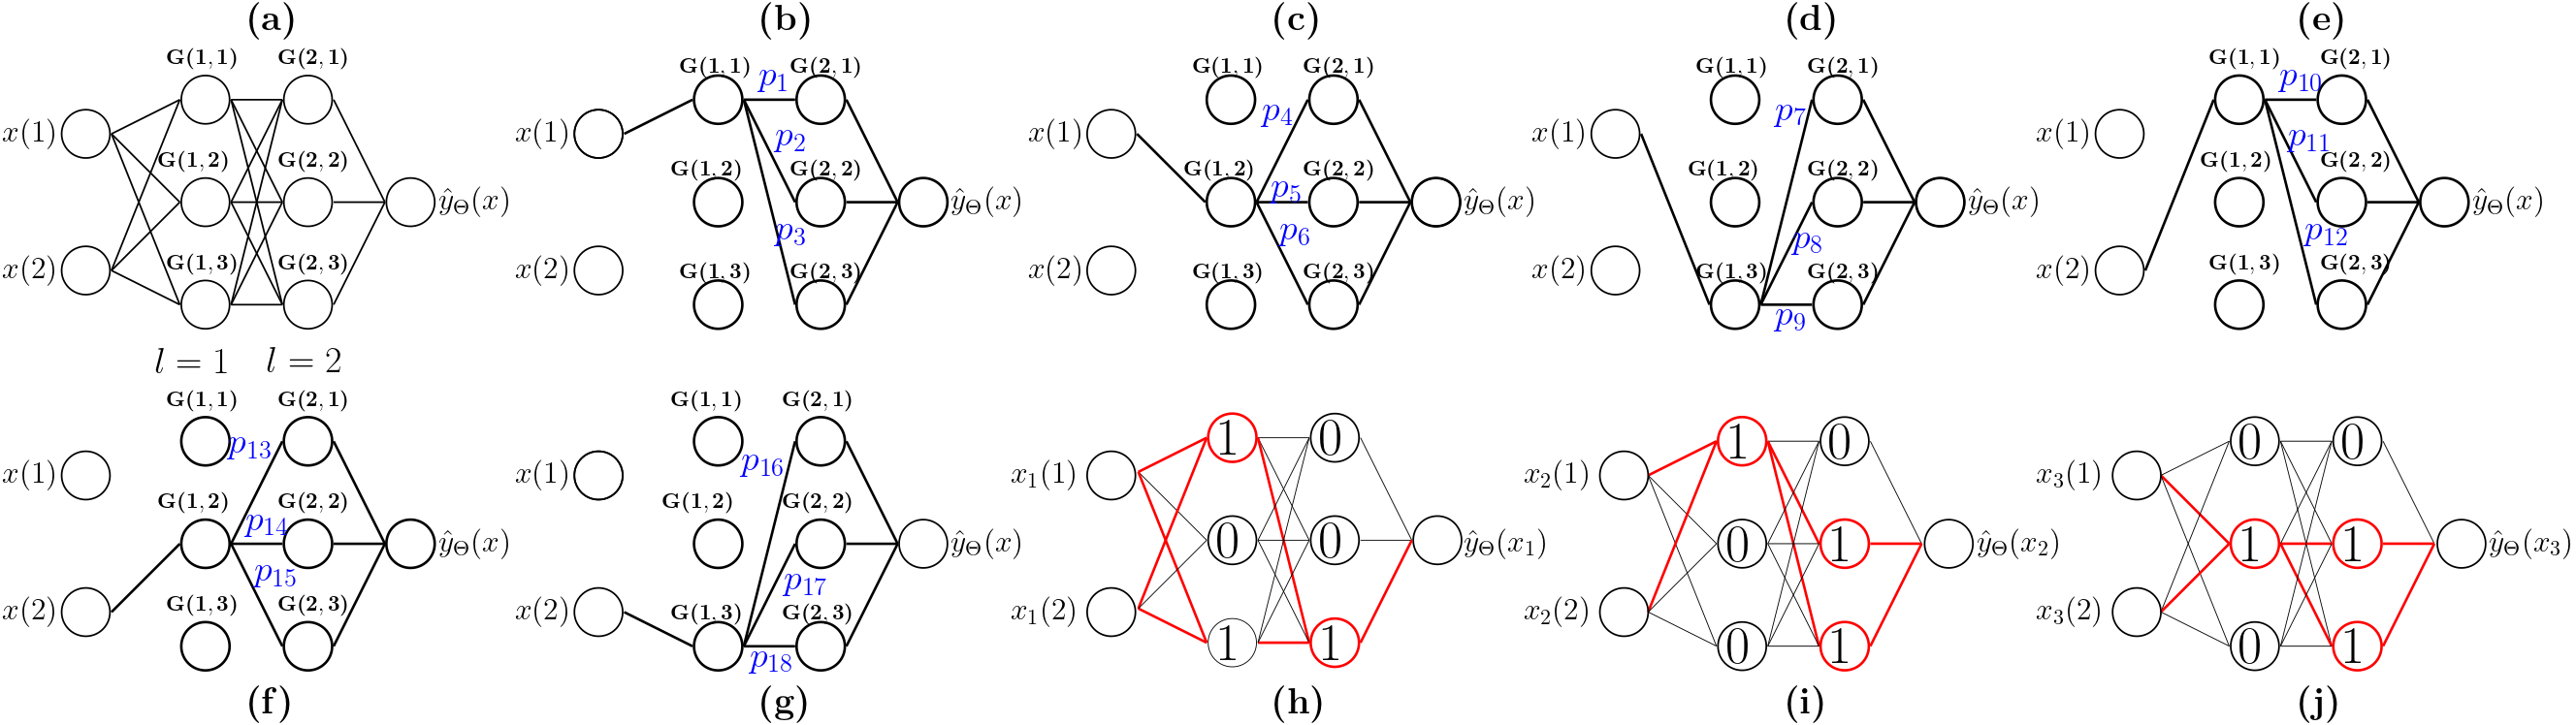
\includegraphics[scale=1]{figs/npf-npk-flipped.png}
}
\centering
%\resizebox{\columnwidth}{!}{
%$\phi_{x}=[x(1)A(x,p_1),\ldots,x(1)A(x,p_{9}),x(2)A(x,p_{10}),\ldots,x(2)A(x,p_{18})]^\top, \phi_{x_1}=[0, 0, x_1(1),0,0, 0, 0,0, x_1(1), 0, 0, x_1(2),0, 0, 0,0, 0, x_1(2)]^\top$
%}
%\resizebox{\columnwidth}{!}{
%$\phi_{x_2}=[0, x_2(1), x_2(1),0,0, 0, 0,0,0, 0, x_2(2), x_2(2),0,0, 0, 0,0,0 ]^\top, \phi_{x_3}=[0, 0,0,0, x_3(1),x_3(1),0,0, 0,0, 0,0,0, x_3(2),x_3(2),0,0, 0 ]^\top$
%}
\begin{minipage}{0.64\textwidth}
%\resizebox{\columnwidth}{!}{
%$\phi_{x}=[x(1)A(x,p_1),\ldots,x(1)A(x,p_{9}),x(2)A(x,p_{10}),\ldots,x(2)A(x,p_{18})]^\top$
%}
%\\
\resizebox{\columnwidth}{!}{
$\phi_{x_1}=[0, 0, x_1(1),0,0, 0, 0,0, x_1(1), 0, 0, x_1(2),0, 0, 0,0, 0, x_1(2)]^\top$
}
\\
\resizebox{\columnwidth}{!}{
$\phi_{x_2}=[0, x_2(1), x_2(1),0,0, 0, 0,0,0, 0, x_2(2), x_2(2),0,0, 0, 0,0,0 ]^\top$
}
\\
\resizebox{\columnwidth}{!}{
$\phi_{x_3}=[0, 0,0,0, x_3(1),x_3(1),0,0, 0,0, 0,0,0, x_3(2),x_3(2),0,0, 0 ]^\top$
}
\end{minipage}
\begin{minipage}{0.25\textwidth}
%\resizebox{\columnwidth}{!}{
,\,$\Lambda=\left[\begin{matrix} 
2 &1& 0 \\
1 &2& 0\\
0 &0& 2
\end{matrix}\right]$
%}
\end{minipage}

\begin{comment}
\begin{minipage}{0.4\textwidth}
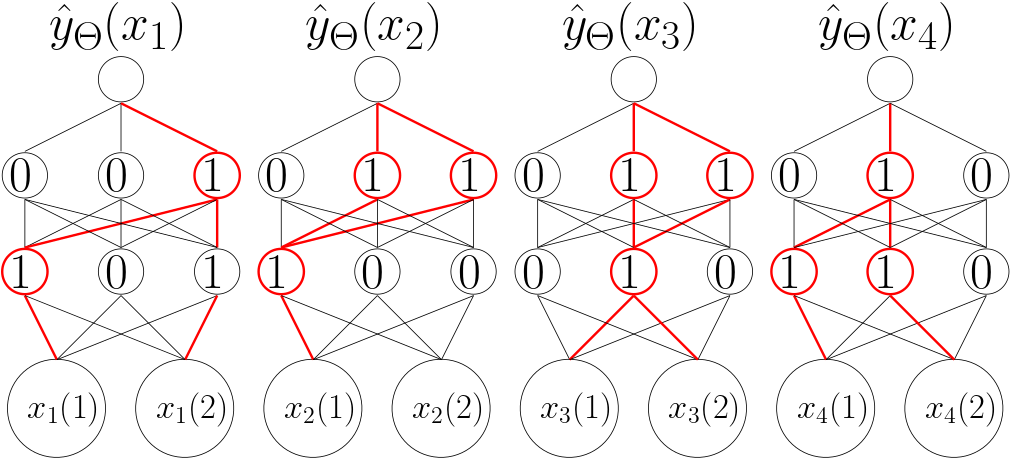
\includegraphics[scale=0.15]{figs/npf-npk.png}
\end{minipage}
\begin{minipage}{0.55\textwidth}
%\resizebox{\columnwidth}{!}{
%$\phi_{x,\Theta}=[x(1)A_{\Theta}(x,p_1),\ldots, x(1)A_{\Theta}(x,p_9),x(2)A_{\Theta}(x,p_{10}),\ldots, x(2)A_{\Theta}(x,p_{18})]^\top$
%}
%\\
\resizebox{\columnwidth}{!}{
$\phi_{x_1,\Theta}=[0, 0, x_1(1),0,0, 0, 0,0, x_1(1), 0, 0, x_1(2),0, 0, 0,0, 0, x_1(2)]^\top$
}
\\
\resizebox{\columnwidth}{!}{
$\phi_{x_2,\Theta}=[0, x_2(1), x_2(1),0,0, 0, 0,0,0, 0, x_2(2), x_2(2),0,0, 0, 0,0,0 ]^\top$
}
\\
\resizebox{\columnwidth}{!}{
$\phi_{x_3,\Theta}=[0, 0,0,0, x_3(1),x_3(1),0,0, 0,0, 0,0,0, x_3(2),x_3(2),0,0, 0 ]^\top$
}
\\
\resizebox{\columnwidth}{!}{
$\phi_{x_4,\Theta}=[0,x_4(1), 0,0, x_4(1),0, 0,0,0,0,x_4(2), 0,0, x_4(2),0, 0,0,0]^\top$
}
\end{minipage}
\end{comment}
%\end{minipage}
\caption{A toy illustration of gates, paths and active sub-networks. The cartoon (\textbf{a}) in the top left corner shows a DNN with $2$ hidden layers, $6$ ReLU gates $G(l,i),l=1,2,i=1,2,3$, $2$ input nodes $x(1)$ and $x(2)$ and an output node $\hat{y}_{\Theta}(x)$. Cartoons (\textbf{b}) to (\textbf{g}) show the enumeration of the paths $p_1,\ldots, p_{18}$. Cartoons (\textbf{h}), (\textbf{i}) and (\textbf{j}) show hypothetical gates for $3$ different hypothetical input examples $\{x_s\}_{s=1}^3 \in\R^2$. In each of the cartoons (\textbf{h}), (\textbf{i}) and (\textbf{j}), the $1/0$ inside the circles denotes the on/off state of the gates, and the bold paths/gates shown in red colour constitute the active sub-network for that particular input example. The NPFs are given by $\phi_{x}=[x(1)A(x,p_1),\ldots,x(1)A(x,p_{9}),x(2)A(x,p_{10}),\ldots,x(2)A(x,p_{18})]^\top$.Here, $\Lambda(1,2)=1$ because paths $p_3$ and $p_{12}$ are both active for input examples $x_1$ and $x_2$ and the input dimension is $2$.}% Here $\tau(s,s',l)$ is the total number of gates in layer $l$ that are $1$ for both inputs $x_s$ and $x_{s'}$.  Here, $\Lambda(1,2)=1$ because paths $p_3$ and $p_{12}$ are both active for input examples $x_1$ and $x_2$ and the input dimension is $2$.}
\label{fig:npkexample}
\end{figure}


\subsection{Neural Path Kernel : Similarity based on active sub-networks}
\begin{comment}
\begin{definition}\label{def:lambda}
For input examples $s, s'\in[n]$ define 

$1.$ $\tau_{\Theta}(s,s',l)\stackrel{def}=\sum_{i=1}^w G_{x_s,\Theta}(l,i)G_{x_{s'},\Theta}(l,i)$ be the number of activations that are ``on'' for both inputs $s,s'\in[n]$ in layer $l\in[d-1]$.

$2.$ $\Lambda_{\Theta}(s,s')\stackrel{def}=\Pi_{l=1}^{d-1}\tau_{\Theta}(s,s',l)$.
\end{definition}
\end{comment}
\begin{definition}\label{def:lambda}
 For input examples $s,s'\in[n]$, define $\A_{\Theta}(s,s')\stackrel{def}=\{p\in[P]\colon A_{\Theta}(x_s,p)= A_{\Theta}(x_{s'},p)=1\}$ to be the set of `active' paths for both $s,s'$  and $\Lambda_{\Theta}(s,s')\stackrel{def}=\frac{|\A_{\Theta}(s,s')|}{d_{in}}$.
\end{definition}
\textbf{Remark:} Owing to the symmetry of a DNN, the same number of active paths start from any fixed input node. In \Cref{def:lambda}, $\Lambda_{\Theta}$ measures the size of the active sub-network as the total number of active paths starting from any fixed input node. For examples $s,s'\in[n],s\neq s'$, $\Lambda_{\Theta}(s,s)$ is equal to the size of the sub-network active for $s$, and $\Lambda_{\Theta}(s,s')$ is equal to the size of the sub-network active for both $s$ and $s'$. For an illustration of NPFs and $\Lambda$ please see \Cref{fig:npkexample}.
%For a given example $s\in[n]$, $\Lambda_{\Theta}(s,s)$ is equal to the total number of active paths for that input example divided by the number of input nodes (i.e., $d_{in}$), and for different input examples $s,s'\in[n]$ it is equal to the total number of paths in the sub-network that is active for both examples $s,s'\in[n]$, divided by the number of input nodes (i.e., $d_{in}$).
\begin{lemma}\label{lm:npk}
Let $H_{\Theta}\stackrel{def}{=}\Phi^\top_{\Theta}\Phi_{\Theta}$ be the NPK matrix, and $\Lambda_{\Theta}\in\R^{n\times n}$ be as in \Cref{def:lambda} . It follows that $H_{\Theta}= \Sigma\odot\Lambda_{\Theta}$, where $\odot$ is  the Hadamard product, and $\Sigma$ is the input Gram matrix.
\end{lemma}
\begin{comment}
\begin{proposition}
For any $s,s'\in[n]$, such that $s\neq s'$ we have: 

$1.$ $\Theta_0\inrdnet$ be a randomised initialisation of weights from a symmetric distribution with zero mean, then $\forall l\in[d-1], \frac{\tau_{\Theta_0}(s,s,l)}{w}\ra\frac{1}{2}$ as $w\ra\infty$, and $\left(\frac{2}{w}\right)^{(d-1)}\Lambda_{\Theta_0}(s,s)\ra1$.

$2.$ $\frac{\tau_{\Theta}(s,s',l)}{\tau_{\Theta}(s,s,l)}\leq 1,\forall l\in[d-1]$, and hence$ \frac{\Lambda_{\Theta}(s,s')}{\Lambda_{\Theta}(s,s)}$ is non-increasing.
\end{proposition}
\end{comment}

\section{Dynamics of Gradient Descent with NPF and NPV Learning}\label{sec:gatedyna}
In \Cref{sec:path}, we mentioned that during gradient descent, the DNN is learning a relation $\hat{y}_{\Theta}=\Phi^\top_{\Theta} v_{\Theta}$, i.e., both the NPFs and the NPV are learnt. In this section, we connect the newly defined quantities, i..e, $\Phi_{\Theta}$ and $v_{\Theta}$ to the NTK matrix $K_{\Theta}$ (see \Cref{prop:ntknew}), and re-write the gradient descent dynamics in \Cref{prop:dnnhard} taking into account of NPF and NPV learning.
%Also, recall that $\psi_{x_s,\Theta}=(\partial_{\theta}\hat{y}_{\Theta}(x_s),\theta\in\Theta)$ and $K_{\Theta}(s,s')=\ip{}$
%In this section, we re-write \Cref{prop:basic} in \Cref{prop:dnnhard,prop:dnnsoft}, wherein, in addition to the dynamics of the weights ($\dot{\Theta}_t$) and the error ($\dot{e}_t$), we also capture the dynamics of the NPF (i.e., dynamics of the gates) and the NPV during GD. %Since the NPFs encode the states of the gates, the dynamics of the gates is accounted by accounting for the dynamics of NPFs.
\begin{comment}
\begin{proposition}
Define $\psiv_{x,\Theta}\stackrel{def}=\left(\ip{\phi_{x,\Theta}, \partial_{\theta} v_{\Theta}},\theta\in\Theta\right)\in\R^{d_{net}}$ and $\psif_{x,\Theta}\stackrel{def}=\left(\ip{\partial_{\theta}\phi_{x,\Theta}, v_{\Theta}},\theta\in\Theta\right)\in\R^{d_{net}}$. It follows that 
$\psi_{x,\Theta}=\psiv_{x,\Theta}+\psif_{x,\Theta}$.
\end{proposition}
\begin{proposition}
In DNNs with ReLU gates, $\psif_{x,\Theta}=0,\forall x\in\R^{d_{in}}, \Theta\in\R^{d_{net}}$.
\end{proposition}
\end{comment}
\subsection{NPV and NPF Learning}
\begin{definition}\label{def:npvgrad}
The gradient of the NPV of path $p$ is defined as $\varphi_{p,\Theta}\stackrel{def}=(\partial_{\theta}v_{\Theta}(p), \theta \in\Theta)\in\R^{d_{net}}$.
\end{definition}
\textbf{Remark} The change of the NPV is given by $\dot{v}_{\Theta_t}(p)=\ip{\varphi_{p,\Theta_t},\dot{\Theta}_t}$, where $\dot{\Theta}_t$ is the change of the weights. We now collect the gradients $\varphi_{p,\Theta}$ of all the paths to define a \emph{value tangent kernel} (VTK). 
\begin{definition}
Let $\nabla_{\Theta}v_{\Theta}$ be a $d_{net}\times P$ matrix of NPV derivatives given by $\nabla_{\Theta}v_{\Theta}=(\varphi_{p,\Theta},p\in[P])$. Define the VTK to be the $P\times P$ matrix given by $\V_{\Theta}=(\nabla_{\Theta}v_{\Theta})^\top(\nabla_{\Theta}v_{\Theta})$.
\end{definition}
\textbf{Remark} An important point to note here is that the VTK is a quantity that is dependent only on the weights. To appreciate the same, consider a deep linear network (DLN) [\citenum{shamir,dudln}] which has identity activations, i.e., all the gates are $1$ for all inputs, and weights. For a DLN and DNN with identical network architecture (i.e., $w$ and $d$), and identical weights, $\V_{\Theta}$ is also identical. Thus, $\V_{\Theta}$ is the gradient based information that excludes the gating information.
%\subsection{NPF Learning}

The NPFs changes at those time instants when any one of the gates switches from $1$ to $0$ or from $0$ to $1$. In the time between two such switching instances, NPFs of all the input examples in the dataset remain the same, and between successive switching instances,  the NPF of at least one of the input example in the dataset changes. In what follows, in \Cref{prop:dnnhard} we re-write \Cref{prop:basic} taking into account the switching instances which we define in \Cref{def:switch}.
\begin{definition}\label{def:switch}
Define a sequence of monotonically increasing time instants $\{T_{i}\}_{i=0}^\infty$ (with $T_0=0$) to be `switching' instants if $\phi_{x_s,\Theta_t}=\phi_{x_s,\Theta_{T_i}},\forall s\in[n],\forall t\in[T_{i},T_{i+1}), i=0,\ldots,\infty$, and  $\forall i=0,\ldots, \infty$ $\exists s(i)\in[n]$ such that $\phi_{x_{s(i)},\Theta_{T_i}}\neq \phi_{x_{s(i)},\Theta_{T_{i+1}}}$.
\end{definition}
\subsection{Gradient Descent}
\begin{proposition}\label{prop:ntknew}
The NTK is given by $K_{\Theta}=\Phi^\top_{\Theta}\V_{\Theta}\Phi_{\Theta}$.
\end{proposition}
\textbf{Remark} $K_{\Theta_t}$ changes during training (i) continuously at all $t\geq 0$ due to $\V_{\Theta_t}$, and (ii) at switching instants $T_{i},i=0,\ldots,\infty$ due to the change in $\Phi_{\Theta_{T_i}}$. We now describe the gradient descent dynamics taking into the dynamics of the NPV and the NPFs.
\begin{comment}
\textbf{Remark:} The NTK matrix is given by $K_{\Theta}(s,s')=\ip{\psi_{x_s,\Theta},\psi_{x_{s'},\Theta}}, s, s'\in[n]$ and can be further decomposed as:
\begin{align}\label{eq:kerneldecomp}
K_{\Theta}(s,s')=\underbrace{{\kv(s,s')}}_{\ip{\psiv_{x_s,\Theta},\psiv_{x_{s'},\Theta}}}+\underbrace{\kf(s,s')}_{\ip{\psif_{x_s,\Theta},\psif_{x_{s'},\Theta}}}+\underbrace{\kc(s,s')}_{\ip{\psiv_{x_s,\Theta},\psif_{x_{s'},\Theta}}+\ip{\psif_{x_s,\Theta},\psiv_{x_{s'},\Theta}}}
\end{align}
\end{comment}
\begin{proposition}\label{prop:dnnhard}
Let $\{T_i\}_{i=0}^\infty$ be as in \Cref{def:switch}. For $t\in[T_{i},T_{i+1})$ and small step-size of GD:
\FloatBarrier
\begin{table}[h]
\centering
\begin{tabular}{ l c l l l }
Weights Dynamics &:  & $\dot{\Theta}_t$&$=$&$-\sum_{s=1}^n \psi_{x_s,\Theta_t}e_t(s)$\\
NPV Dynamics&: & $\dot{v}_{\Theta_t}(p)$&$=$&$\ip{\varphi_{p,\Theta_t},\dot{\Theta}_t},\forall p\in[P]$\\
%Kernel &:& $K_{\Theta_t}$&$=$&$\Phi^\top_{\Theta_{T_i}}\V_{\Theta_t}\Phi_{\Theta_{T_i}}$\\
Error Dynamics&: & $\dot{e}_t$&$=$&$-K_{\Theta_t}e_t$, where $K_{\Theta_t}=\Phi^\top_{\Theta_{T_i}}\V_{\Theta_t}\Phi_{\Theta_{T_i}}$\\
\end{tabular}
\end{table}
\end{proposition}
\begin{proposition}\label{prop:condition}
 $\rho_{min}(K_{\Theta})\leq \rho_{\min}(H_{\Theta})\rho_{\max}\left(\V_{\Theta}\right)$.
\end{proposition}
\textbf{Remark} For the NTK to be well conditioned, it is necessary for the NPK to be well conditioned. This is quite intuitive, in that, the closer two inputs are, the closer are their NPFs, and it is harder to train the network to produce arbitrarily different outputs for such inputs that are very close to one another.
\begin{comment}
%\subsection{Gradient Descent Dynamics in DNN with Soft-ReLU}
We can further simplify (i.e., without using switching instances) the dynamics of GD by using a `soft-ReLU' gate $\gamma_{sr}(q)=\frac{1}{\left(1+\exp(-\beta \cdot q)\right)}, \beta>0$, whose derivative its pre-activation is given by $\partial_{q}\gamma_{sr}(q)=\frac{\beta}{\left(1+\exp(\beta\cdot q)\right)\left(1+\exp(-\beta\cdot q)\right)}$. 
\begin{proposition}\label{prop:dnnsoft} For an infinitesimally small step-size of GD, the error dynamics  of a DNN with soft-ReLU gates is given by:
\FloatBarrier
\begin{table}[h]
\centering
\begin{tabular}{| l | lll |}\hline
Weights  & $\dot{\Theta}_t$&$=$&$-\sum_{s=1}^n \psi_{x_s,\Theta_t}e_t(s)=\sum_{s=1}^n (\psiv_{x_s,\Theta_t}+\psif_{x_s,\Theta_t})e_t(s)$\\
NPF & $\dot{\phi}_{x_s,\Theta_t}(p)$&$=$&$x(\I_0(p))\sum_{\theta\in\Theta}\partial_{\theta}A_{\Theta_t}(x_s,p)\dot{\theta}_t,\forall p\in[P], s\in[n]$\\
NPV & $\dot{v}_{\Theta_t}(p)$&$=$&$\sum_{\theta\in\Theta}\partial_{\theta}v_{\Theta_t}(p)\dot{\theta}_t,\forall p\in[P]$\\
Error & $\dot{e}_t$&$=$&$-K_{\Theta_t}e_t$, where $K_{\Theta}=\kv+\kf+\kc$\ \\\hline
\end{tabular}
\end{table}
\end{proposition}
\textbf{Remark:} Thanks to the soft-ReLU trick, we are able to capture the NPF learning via $\dot{\phi}_{x_s,\Theta_t}$ term.
\end{comment}
\section{Deep Gated Networks: Decoupling Neural Path Feature and Value}\label{sec:decoupled}
\begin{comment}
We encoded the gating information in the NPFs, and we saw that the decompositions of $\psi_{x,\Theta}=\psiv_{x,\Theta}+\psiv_{x,\Theta}$ and $K_{\Theta}=\kv+\kf+\kc$ captured terms related to NPF learning (and hence gating dynamics). However, from \Cref{prop:basic}, it is only known that $K_{\Theta_t}$ as a whole dictates GD dynamics. Thus, in order to ascertain that NPF learning terms $\psiv$, $\kf$ indeed make a difference, we should separate them out (from $\psi$and $K_{\Theta}$), and measure the generalisation performance with and without the NPF learning terms. This separation can be achieved by a deep gated network (see \Cref{fig:dgn} below for details) having two networks of identical architecture namely i) a feature network parameterised by $\Tg\inrdnet$, that holds gating information, and hence the NPFs and ii) a value network that holds the NPVs parameterised by $\Tv\inrdnet$.  By making $\Tg\inrdnet$ trainable/non-trainable, we can \emph{enable/disable} the NPF gradient, which gives rise to the following two modes of operating a DGN:
\end{comment}
In order to ascertain that  NPF learning indeed makes a difference, we should measure the generalisation performance with and without NPF learning. This can be achieved by a deep gated network (see \Cref{fig:dgn} below for details) having two networks of identical architecture namely i) a feature network parameterised by $\Tg\inrdnet$, that holds gating information, and hence the NPFs and ii) a value network that holds the NPVs parameterised by $\Tv\inrdnet$.  In what follows, we let $\Tdgn=(\Tg,\Tv)\in\R^{2_{dnet}}$to denote the combined parameters of a DGN. By making $\Tg\inrdnet$ trainable/non-trainable, we can \emph{enable/disable} the NPF gradient, which gives rise to the following two modes of operating a DGN:

$1.$ \textbf{Fixed NPF (FNPF):} Here, $\Tg_t=\Tg_0,\forall t\geq 0$, i.e., $\Tg\inrdnet$ is non-trainable. Thus the DGN learns the relation $\hat{y}_{\Tdgn}=\Phi^\top_{\Tg_0}v_{\Tv}$, where $\Phi_{\Tg_0}\in \R^{P\times n}$ is a fixed NPF matrix, and $v_{\Tv}$ is learned via gradient descent on $\Tv\inrdnet$.

$2.$ \textbf{Decoupled NPF Learning (DNPFL):} Here both $\Tg\inrdnet$ and $\Tv\inrdnet$ are trained, and the DGN learns the relation $\hat{y}_{\Tdgn}=\Phi^\top_{\Tg}v_{\Tv}$. In comparison to \eqref{eq:npfnpv}, here we have two parameters $\Tg\inrdnet$ and $\Tv\inrdnet$ as opposed to a single $\Theta\inrdnet$ in \eqref{eq:npfnpv}.

\textbf{Note:} FNPF and DNPFL are idealised modes to understand the role of gates, and not alternate proposals to replace standard DNNs with ReLU activations. 
\begin{figure}[h] 
\begin{minipage}{0.70\columnwidth}
\resizebox{\columnwidth}{!}{
\begin{tabular}{|l|l|l|}\hline
Layer& Feature Network (NPF)& Value Network (NPV)\\
Input & $z^{\text{F}}_{x,t}(0)=x$ &$z^{\text{V}}_{x,t}(0)=x$ \\
Activation & $q^{\text{F}}_{x,t}(l)={\Tg_t(l)}^\top z^{\text{F}}_{x,t}(l-1)$& $q^{\text{V}}_{x,t}(l)={\Tv_t(l)}^\top z^{\text{V}}_{x,t}(l-1)$\\
Hidden &$z^{\text{F}}_{x,t}(l)=\chi^{\text{F}}\left(q^{\text{F}}_{x,t}(l)\right)$& $z^{\text{V}}_{x,t}(l)=q^{\text{V}}_{x,t}(l)\odot G_{x,t}(l)$ \\
Output & None &$\hat{y}_t(x)={\Tv(d)}^\top z^{\text{V}}_{x,t}(d-1)$\\\hline
\multicolumn{3}{|l|}{Gating Values:\quad$ G_{x,t}(l)= \gamma_{r}\left(q^{\text{F}}_{x,t}(l)\right)\quad$or $G_{x,t}(l)= \gamma_{sr}\left(q^{\text{F}}_{x,t}(l)\right)$}\\\hline
\end{tabular}
}
\end{minipage}
\begin{minipage}{0.29\columnwidth}
\resizebox{\columnwidth}{!}{
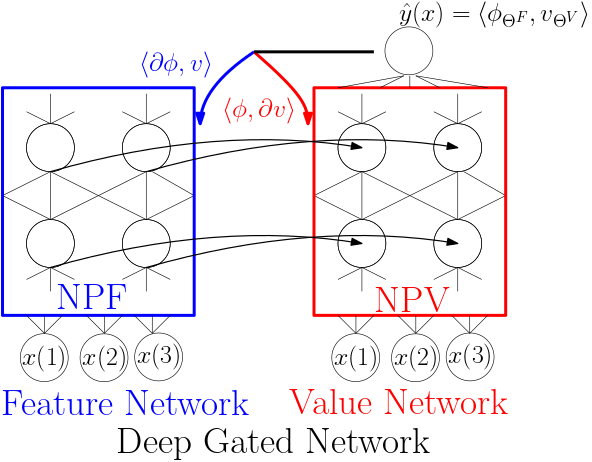
\includegraphics[scale=0.5]{figs/nntwin-blck.png}
}
\end{minipage}
\caption{Deep gated network (DGN) setup.  The pre-activations $q^{\text{F}}_{x,t}(l)$ of layer $l\in[d-1]$ from the feature network are used to derive the gating values $G_{x,t}(l)$ of layer $l\in[d-1]$. }
\label{fig:dgn}
\end{figure}
\begin{comment}
Note that, the feature network uses $\chi^{\text{F}}$ as the activation function, which can be a standard ReLU activation, i.e., $\chi^{\text{F}}=\chi_r$. The pre-activations $q^{\text{F}}_{x,t}(l)$ of layer $l\in[d-1]$ from the feature network are used to derive the gating values $G_{x,t}(l)$ of layer $l\in[d-1]$. The gating values can be obtained from either a ReLU gate $\gamma_r$ or a soft-ReLU gate $\gamma_{sr}$. The process of separating the NPFs and the NPVs decouples the value and the feature gradients. In a DGN, the value gradient $\psiv_{x,\Tdgn}$ flows through the value network and the feature gradient $\psif_{x,\Tdgn}$flows through the feature network. 
\end{comment}
\begin{proposition}[Gradient Dynamics in a DGN]\label{prop:dgn} Let $\psif_{x,\Tdgn}\stackrel{def}=\nabla_{\Tg}\hat{y}_{\Tdgn}(x) \in \R^{d_{net}}$, $\psiv_{x,\Tdgn}\stackrel{def}=\nabla_{\Tv}\hat{y}_{\Tdgn}(x) \in \R^{d_{net}}$. Let $K^{\text{V}}_{\Tdgn}$ and $K^{\text{F}}_{\Tdgn}$ be $n\times n$ matrices with entries $K^{\text{V}}_{\Tdgn}(s,s')=\ip{\psiv_{x_s,\Tdgn},\psiv_{x_{s'},\Tdgn}}$ and $K^{\text{F}}_{\Tdgn}(s,s')=\ip{\psif_{x_s,\Tdgn},\psif_{x_{s'},\Tdgn}}$. For infinitesimally small step-size of GD, the error dynamics in a DGN (in the DNPFL  and FNPF modes) is given by:
\FloatBarrier
\begin{table}[h]
\resizebox{\columnwidth}{!}{
\begin{tabular}{| l | l l l | l |}\hline
	Dynamics&		&&DNPFL& FNPF\\\hline
		&		&&& \\
Weight  & $\dot{\Theta}^{\text{V}}_t$&$=$&$-\sum_{s=1}^n \psiv_{x,\Tdgn_t}e_t(s),\dot{\Theta}^{\text{F}}_t=-\sum_{s=1}^n \psif_{x,\Tdgn_t}e_t(s)$ & $\dot{\Theta}^{\text{V}}_t$ same as (DNFPL),  $\dot{\Theta}^{\text{F}}_t=0$\\
NPF & $\dot{\phi}_{x_s,\Tg_t}(p)$&$=$&$x(\I_0(p))\sum_{\tg\in\Tg}\partial_{\tg}A_{\Tg_t}(x_s,p)\dot{\theta}^{\text{F}}_t,\forall p\in[P], s\in[n]$& $\dot{\phi}_{x_s,\Tg_t}(p)=0$\\
NPV & $\dot{v}_{\Tv_t}(p)$&$=$&$\sum_{\tv\in\Tv}\partial_{\tv}v_{\Tv_t}(p)\dot{\theta}^{\text{V}}_t,\forall p\in[P]$ & $\dot{v}_{\Tv_t}(p)$ same as DNPFL\\
%Kernel & $K_{\Tdgn}$&$=$&$K^{\text{V}}_{\Tdgn}+ K^{\text{F}}_{\Tdgn}$ & $K_{\Tdgn}=K^{\text{V}}_{\Tdgn}$ \\\hline
Error & $\dot{e}_t$&$=$&$-\left(K^{\text{V}}_{\Tdgn}+ K^{\text{F}}_{\Tdgn}\right)e_t$  & $\dot{e}_t=-\left(K^{\text{V}}_{\Tdgn}\right)e_t$ \\\hline
\end{tabular}
}
\end{table}
\end{proposition}
\textbf{Remark:} The gradient dynamics in a DGN specified in \Cref{prop:dgn} is similar to the gradient dynamics in a DNN specified in \Cref{prop:dnnhard}. Important difference is that in a DGN there are $2d_{net}$ parameters, and hence the NTF $\psi_{x,\Theta}=(\psif_{x,\Theta},\psiv_{x,\Theta})\in\R^{2d_{net}}$, wherein, $\psiv_{x,\Tdgn}\inrdnet$ flows through the value network and $\psif_{x,\Tdgn}\inrdnet$ flows through the feature network. %As a result $\kc=0$. Note that in the FNPF mode of the DGN, since $\Tg\inrdnet$ are non-trainable $\psif=0$, and hence $\dot{\phi}=0$ and $\kf=0$.
\section{Learning with Fixed NPFs: Role Of Active Sub-Networks}\label{sec:infomeasure}
In this section, we provide theoretical justification for ``Claim I'', i.e., the active sub-networks are fundamental entities in DNNs. 
% Consider a DNN parameterised by $\bar{\Theta}\inrdnet$. At randomised initialisation, we can obtain random NPFs $\Phi_{\bar{\Theta}_0}$, and after training for $T$ epochs, and we can obtained learnt NPFs $\Phi_{\bar{\Theta}_T}$. One way to measure the difference between random NPFs and learnt NPFs is to keep the respective NPFs fixed (by storing them in a feature network) and only learn the NPVs. We now present an assumption and result on learning with fixed NPFs.
%\begin{comment}
\begin{definition}\label{def:gateinfo}
Define the measure of information stored in the gates of a \emph{DNN} with parameter $\bar{\Theta}\inrdnet$ to be the generalisation performance of a \emph{DGN} with identical architecture operated in the \emph{FNPF} mode whose $\Tg_0=\bar{\Theta}$ are non-trainable, and $\Tv\inrdnet$ are trained.
\end{definition}
Consider a DNN parameterised by $\bar{\Theta}\inrdnet$. At randomised initialisation, we can obtain random NPFs $\Phi_{\bar{\Theta}_0}$, and after training for $T$ epochs, and we can obtain learnt NPFs $\Phi_{\bar{\Theta}_T}$. 
%Suppose we train a standard DNN for $T$ epochs, and say the parameter at end of training is $\bar{\Theta}_T$. In this case, the relation learnt is $\hat{y}_{\bar{\Theta}_T}=\Phi_{\bar{\Theta}_T}v_{\bar{\Theta}_T}$. 
Thus, while measuring information in the gates of this trained DNN, as per \Cref{def:gateinfo}, we are retaining $\Phi_{\bar{\Theta}_T}$ by storing the weights as $\Tg_0=\bar{\Theta}_T$ in the feature network, and discarding $v_{\bar{\Theta}_T}$, and re-training $\Tv$ to learn a new relation $\hat{y}_{\Tdgn}=\Phi^\top_{\Tg_0}v_{\Tv}=\Phi^\top_{\bar{\Theta}_T}v_{\Tv}$. Similarly, in the case of random NPFs we are learning the relation, $\hat{y}_{\Tdgn}=\Phi^\top_{\Tg_0}v_{\Tv}=\Phi^\top_{\bar{\Theta}_0}v_{\Tv}$. In what follows, we use $H_{\text{FNFP}}$ to refer to $H_{\Tg_0}$.
%\end{comment}
\begin{assumption}\label{assmp:main}
(i) $\Tv_0\inrdnet$ is statistically independent of the fixed NPFs (stored in $\Tg_0\inrdnet$ of the feature network), (ii) $\Tv_0$ are sampled i.i.d from symmetric Bernoulli over $\{-\sigma,+\sigma\}$.
\end{assumption}
%\textbf{Remark:} Thus at initialisation as per \Cref{assmp:main} the NPFs and NPV are statistically independent. In what follows, we use $H_{\text{FNFP}}$ to refer to $H_{\Tg_0}$.
\begin{theorem}\label{th:main} Under \Cref{assmp:main}, as $w\ra\infty$, $K_{\Tdgn_0}\ra K^{(d)}_{\text{FNPF}} =d\cdot \sigma^{2(d-1)} H_{\text{FNPF}}$.%=d\cdot \Sigma\odot\bar{\Lambda}_{\Tg_0}$, where $\bar{\Lambda}_{\Tg_0}=\sigma^{2(d-1)}\Lambda_{\Tg_0} $.
\end{theorem}
\begin{comment}
\begin{theorem}\label{th:main} Let be $H_{\Tg_0}\stackrel{def}= \Phi^\top_{\Tg_0}\Phi_{\Tg_0}$ be the NPK matrix. As $w\ra\infty$, $K_{\Tdgn_0}\ra d \sigma^{2(d-1)} H_{\Tg_0} $.
%(ii) In addition, if ${4d}/{w^2}<1$, then $Var\left[K_0\right]\leq O\left(d^2_{in}\sigma^{4(d-1)}\max\{d^2w^{2(d-2)+1}, d^3w^{2(d-2)}\}\right)$.
\end{theorem}
\end{comment}
$\bullet$ \textbf{Active Sub-Network:} From previous results \cite{arora2019exact}, it follows that as $w\ra\infty$, the optimisation and generalisation properties of the fixed NPF learner can be tied down to the infinite width NTK of the FNPF learner $K^{(d)}_{\text{FNPF}}$ and hence to $H_{\text{FNPF}}$ (treating $d\sigma^{2(d-1)}$ as a scaling factor).  We can further breakdown $H_{\text{FNPF}}=\Sigma\odot{\Lambda}_{\text{FNPF}}$, where $\Lambda_{\text{FNPF}}=\Lambda_{\Tg_0}$. This justifies ``Claim I''. 

$\bullet$ $K^{(d)}$ in prior works [\citenum{ntk,arora2019exact,cao2019generalization}] essentially becomes $K^{(d)}_{\text{FNPF}}$ under \Cref{assmp:main}.  To understand this, let us consider a DNN with weights $\Theta\inrdnet$. From  [\citenum{ntk,arora2019exact,cao2019generalization}] it follows that under randomised initialisation of $\Theta_0\inrdnet$ as $w\ra\infty$ the NTK of the DNN  $K_{\Theta_0}\ra K^{(d)}$. The simplification of $K^{(d)}$ to $K^{(d)}_{\text{FNPF}}$ in \Cref{th:main} occurs when we copy these random NPFs corresponding to $\Theta_0\inrdnet$ into the feature network and keep them fixed, i.e., $\Tg_t=\Tg_0=\Theta_0\inrdnet,t\geq 0$, and train $\Tv\inrdnet$ with initialisation as per \Cref{assmp:main}.
 
 $\bullet$ \textbf{Choice of $\sigma$:} In the case of random NPFs obtained by initialising $\Tg_0$ at random by sampling from a symmetric distribution, we expect $\frac{w}2$ gates to be on every layer, so $\sigma=\sqrt{\frac{2}{w}}$ is a normalising choice, in that, the diagonal entries of $\sigma^{2(d-1)}{\Lambda}_{\text{FNPF}}(s,s)\approx 1$ in this case.

$\bullet$ We discuss a more detailed version of \Cref{th:main} in the Appendix, where we discuss the role of width and depth on a pure memorisation task.

\section{Experiments: Fixed NPFs, NPF Learning and Verification of Claim II}\label{sec:experiments} 
In this section, we justify ``Claim II'', i.e., active sub-networks learning is key for generalisation. Since the active sub-network are encoded in the NPFs, we verify the claim by comparing different network settings which vary in their NPF learning capabilities. We resolve the open question of \cite{arora2019exact} mentioned in \Cref{sec:background}, by providing an empirical explanation for the performance gain of finite width CNN over the pure kernel method based on the exact infinite width CNTK.\\
\textbf{Networks for Comparison:} The performance of the following networks on standard MNIST and CIFAR-10 datasets will be used for comparison: (i) fixed random (FRNPF): in the DGN, we randomly initialise both $\Tg_0,\Tv_0$, make $\Tg$ \emph{non-trainable} and train only $\Tv$ , (ii) fixed learnt (FLNPF): we initialise $\Tv_0$ randomly, and copy weights from a pre-trained ReLU network (of identical architecture) into $\Tg_0$. Similar to FR case, $\Tg$ is non-trainable and only $\Tv$ is trained (iii) decoupled learning (DNPFL):  we randomly initialise both $\Tg_0,\Tv_0$, and train both $\Tg$ and $\Tv$, (iv) ReLU: Standard DNNs/CNNs with ReLU.  We will also use the numerical results reported in \cite{arora2019exact}.\\
%The results of our experiments on CIFAR-10 (please look at the \Cref{tb:npfs} for complete results in CIFAR-10 as well as MNIST) that supports ``Claim II' can be summarised as below:
$1.$ \textbf{Finite Vs Infinite width alone is not enough to explain the performance gain of CNN:} Both FRNPF and ReLU are finite width networks. However, performance of FRNPF is  approximately $67\%$ which is worse than CNTK of \cite{arora2019exact} whose performance is $77.43\%$, and the performance of our CNN architecture with \emph{global-average-pooling} (GCONV in \Cref{tb:npfs}) is $80.34\%$. We trained FRNPF with independent initialisation (II), where $\Tg_0$ and $\Tv_0$ are statistically independent, and dependent initialisation (DI), where $\Tg_0=\Tv_0$. FRNPF (II) and FRNPF (DI) were close in our experiments (see columns $4$ and $5$ in \Cref{tb:npfs}). Further, both FRNPF (DI) and ReLU start with the same NTK matrix at initialisation. If finite width was the sole reason for the better performance then even FRNPF (II), (DI) should have performed better than CNTK in the experiments, and they did not. Thus, finite width alone does not explain the performance gain of CNN over CNTK.\\
$2.$ \textbf{NPF Learning Vs No NPF Learning  is key to explain the performance gain of CNN:} FLNPF with weights copied from a fully trained ReLU performs close to $79.68\%$ which is almost as good as ReLU's $80.43\%$ (see FLNP column in \Cref{tb:npfs}). Further, NPFs are learnt continuously during the training, and the performance gap between FRNPF and ReLU is continuous. In the case of CIFAR-10, we trained a GCONV network (parameterised by $\bar{\Theta}$) for $60$ epochs, and we obtained $6$ different weights at various \emph{stages} of the training process. Stage $1$: $\bar{\Theta}_{10}$, stage $2$: $\bar{\Theta}_{20}$, stage $3$: $\bar{\Theta}_{30}$, stage $4$: $\bar{\Theta}_{40}$, stage $5$: $\bar{\Theta}_{50}$, stage $6$: $\bar{\Theta}_{60}$. We copy these weights obtained at various stages of training to setup $6$ different FLNPFs, i.e., FLNPF-$1$ to FLNPF-$6$. We observe that the performance of FLNPF-$1$ to FLNPF-$6$ increases monotonically, with FLNPF-$1$ performing $72\%$ which is better than FRNPF (i.e., $67.08\%$),  and FLNPF-$6$ performing as well as ReLU (see left most plot in \Cref{fig:dynamics}). The performance of CNTK of \cite{arora2019exact} is $77.43\%$. Thus, through its various stages, the FLNPF starts from below $77.43\%$ and surpasses to reach $79.68\%$, which implies performance gain of CNN is due to learning of NPFs.\\
%Since from \Cref{th:main} we know that the generalisation performance of the fixed NPF learner is characterised by its NPK, and the fact that FLNPF almost recovers the performance of ReLU, we observe that \emph{almost all the information learnt by a standard ReLU DNN is stored in its gates}. 
\begin{figure}
\centering
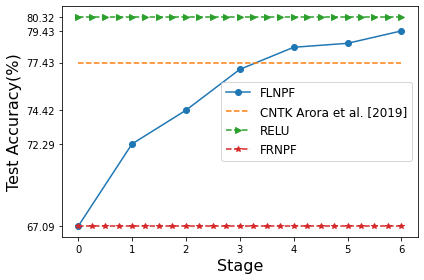
\includegraphics[scale=0.23]{figs/gap.png}
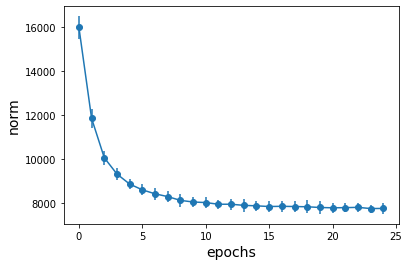
\includegraphics[scale=0.23]{figs/path-gram.png}
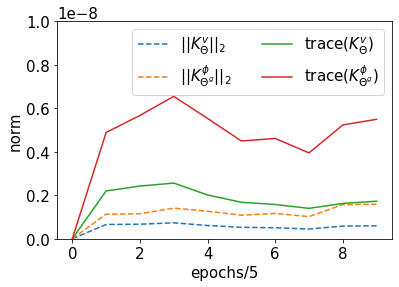
\includegraphics[scale=0.23]{figs/kvkphi.png}
\caption{Dynamics of NPF Learning. }
\label{fig:dynamics}
\end{figure}
$3.$ \textbf{Dynamics of active sub-networks during training:} We considered ``Binary''-MNIST data set with two classes namely digits $4$ and $7$, with the labels taking values in $\{-1,+1\}$ and squared loss. We trained a fully connected (FC) network ($w=100$, $d=5$). Let $\widehat{H}_{\Theta_t}=\frac{1}{trace(H_{\Theta_t})}H_{\Theta_t}$ be the normalised NPK matrix. For a subset size, $n'=200$ ($100$ examples per class) we plot $\nu_t=y^\top (\widehat{H}_{\Theta_t})^{-1} y$, (where $y\in\{-1,1\}^{200}$ is the labelling function), and observe that $\nu_t$ reduces as training proceeds (see middle plot in \Cref{fig:dynamics}). Note that, $\nu_t=\sum_{i=1}^{n'}(u_{i,t}^\top y)^2 (\hat{\rho}_{i,t})^{-1}$, where $u_{i,t}\in \R^{n'}$ are the orthonormal eigenvectors of $\widehat{H}_{\Theta_t}$ and $\hat{\rho}_{i,t},i\in[n']$ are the corresponding eigenvalues. Since $\sum_{i=1}^{n'}\hat{\rho}_{i,t}=1$, the only way $\nu_t$ reduces is when more and more energy gets concentrated on $\hat{\rho}_{i,t}$s for which $(u_{i,t}^\top y)^2$s are also high. Since $H_{\Theta_t}=\Sigma\odot \Lambda_{\Theta_t}$, only $\Lambda_{\Theta_t}$ is learnt during training.\\
$4.$ \textbf{Decoupled learning} of NPFs also performed better than FRNPFs (see column DNPFL in \Cref{tb:npfs}). This demonstrates the fact that NPFs can also be learnt in `stand alone' manner. In this case, the NTK is given by $K_{\Tdgn}=K^{\text{V}}_{\Tdgn}+K^{\text{F}}_{\Tdgn}$. For MNIST, we compared $K^{\text{V}}_{\Tdgn}$ and $K^{\text{F}}_{\Tdgn}$ (calculated using $100$ examples in total with $10$ examples per each of the $10$ classes) using their trace and Frobenius norms, and we observe that $K^{\text{V}}_{\Tdgn}$ and $K^{\text{F}}_{\Tdgn}$ are in the same scale (see right plot in \Cref{fig:dynamics}), which is perhaps pointing to the fact that both $K^{\text{F}}_{\Tdgn}$ and $K^{\text{F}}_{\Tdgn}$ are equally important for obtaining good generalisation performance. In DNPFL, we can separately study the kernel $K^{\text{F}}_{\Tdgn}$ responsible for NPF learning, an interesting future research direction.
%\FloatBarrier
 \begin{table}
\resizebox{\columnwidth}{!}{
\begin{tabular}{|c|c|c|c|c|c|c|c|}\hline
Arch			&Optimiser	&Dataset		&FRNPF (II) 			&FRNPF (DI)			&DNPFL					&FLNPF						&ReLU\\\hline
FC			&SGD		&MNIST 		&$95.85\pm0.10$		&$95.85\pm0.17$		&$97.86\pm0.11$			&$97.10\pm0.09$				&$97.85\pm0.09$\\\hline
FC			&Adam		&MNIST 		&$96.02\pm0.13$		&$96.09\pm0.12$		&$\mathbf{98.22\pm0.05}$	&$\mathbf{97.82\pm0.02}$		&$\mathbf{98.14\pm0.07}$\\\hline
VCONV		&SGD		&CIFAR-$10$	&$58.92\pm0.62$		&$58.83\pm0.27$ 		&$63.21\pm0.07$			&$63.06\pm0.73$				&$67.02\pm0.43$\\\hline
VCONV		&Adam		&CIFAR-$10$	&$64.86\pm1.18$		&$64.68\pm0.84$		&$\mathbf{69.45\pm0.76}$	&$\mathbf{71.4\pm0.47}$			&$\mathbf{72.43\pm0.54}$\\\hline
GCONV	&SGD		&CIFAR-$10$	&$67.36\pm0.56$		&$66.86\pm0.44$		&$\mathbf{74.57\pm0.43}$			&$\mathbf{78.52\pm0.39}$				&$\mathbf{78.90\pm0.37}$\\\hline
GCONV	&Adam		&CIFAR-$10$	&$67.09\pm0.58$		&$67.08\pm0.27$		&$\mathbf{77.12\pm0.19}$	&$\mathbf{79.68\pm0.32}$		&$\mathbf{80.43\pm0.35}$\\\hline
\end{tabular}
}
\caption{Shows the generalisation performance of  different NPFs learning settings. The values in the table are averaged over $5$ runs. Here, FC is a fully connected network with $w=100$ and $d=5$. VCONV and GCONV denote Vanilla CNN and CNN with GAP respectively. Please check \Cref{sec:expsetup} for details on architecture of VCONV and GCONV, and the hyper-parameters.}
\label{tb:npfs}
\end{table}


%\section{Broader Impact}
Deep neural networks are still widely regarded as blackboxes. The standard and accepted view on the inner workings of  deep neural networks is the `layer-by-layer' viewpoint:  as the input progresses through the hidden layers, features at different levels of abstractions are learnt. This paper deviates from the standard `layer-by-layer' viewpoint, in that, it breaks down the deep neural network blackbox into its constituent paths: different set of paths get fired for different inputs, and the output is the summation of the contribution from individual paths. This makes the inner workings of deep neural networks interpretable, i.e., each input is remembered in terms of the active sub-network of the paths that get `fired' for that input, and learning via gradient descent amounts to `rewiring' of the paths. The paper also analytically connects this sub-network and path based view to the recent kernel based interpretation of deep neural networks, and furthers the understanding of feature learning in deep neural networks. We believe that these better insights into the working of DNNs  can potentially lead to foundational algorithmic development in the future.


%\input{supp}

\section{Related Work}
\setcitestyle{authoryear}
\cite{ntk} showed the NTK to be the central quantity in the study of generalisation properties of infinite width DNNs. \cite{jacot2019freeze} identify two regimes that occur at initialisation in fully connected DNNs as the width increases to infinity namely i) \emph{freeze:} here, the (scaled) NTK converges to a constant and hence leads to slow training,  and  ii) \emph{chaos:} here, the NTK converges to Kronecker delta and hence hurts generalisation. \cite{jacot2019freeze} also suggest that for good generalisation it is important to operate the DNNs at the edge of the freeze and the chaos regimes. \cite{arora2019exact} proposed pure kernel method based on the infinite width CNTK (NTK of convolutional neural network) and showed that it out performed state-of-the-art kernel methods by $10\%$. \cite{arora2019exact} also noted a performance gain (about $5-6\%$) of the CNNs over the CNTK.  However, it was also noted by \cite{arora2019exact,lee2019wide} that random NTFs obtained from finite width neural networks do not perform as well as their limiting infinite width counterparts. 
\cite{arora,cao2019generalization} provided generalisation bounds with the NTK norm. \cite{dudnn} use the NTK to show that over-parameterised DNNs trained by gradient descent achieve zero training error. \cite{dudln,shamir,ganguli} studied deep linear networks. Since deep linear networks are special cases of deep gated networks, \Cref{th:main} of our paper also provides an expression for the NTK at initialisation of deep linear networks. To see this, in the case of deep linear networks, all the gates are always $1$ for all input examples, and $\Lambda_{\Theta}$ will be a matrix whose entries will be $w^{(d-1)}$.

The results in our paper are complementary to the prior NTF/NTK based works, in that, the NPK and NPFs are zeroth order kernel and features respectively. In contrast, the NTF is the gradient of the network output with respect to the weights of the network and hence the NTF/NTK are essentially first order quantities. The fixed NPF regime is different from the NTK regime and the freeze/chaos regimes studied in prior works, in that, in the fixed NPF setting the gates are controlled by a separate feature network.

Gated linearity was studied recently by \cite{sss}, where single layered gated networks were considered. In terms of the work in our paper, \cite{sss} consider the fixed NPF setting with random NPFs of a single layer network. In contrast to the work by \cite{sss}, in this paper we considered DGN of depth $d$, and we also showed (using the DNPFL setting) that by gradient descent on the parameters of the feature and the value network we can learn the NPFs leading to better generalisation than learning with the fixed random NPFs. We believe that handling of depth $d$ networks, identification and the use of novel quantities namely NPFs, NPK and, the role of NPF learning in generalisation amount to significant progress in comparison to \cite{sss}. 

The role of gates was also empirically studied by \cite{srivastava2014understanding}, where the active sub-networks are called as \emph{locally competetive} networks. They encode the active subnetwork information in a sub-mask which is bit string that encodes the $0/1$ state of the all the gates. The sub-masks were then visualised using t-SNE. The visualisation showed that the ``subnetworks active for examples of the same class are much more similar to each other compared to the ones activated for the examples of different classes''. \cite{balestriero2018spline} show the connection between $\max$-affine linearity and DNN with ReLU activations. \cite{neyshabur2015path} used the notion of paths to define a \emph{path-norm} based gradient descent procedure. 
\section{Conclusion}
\begin{comment}
Optimisation and generalisation of DNNs has been an important question in machine learning. Prior works have considered the \emph{neural tangent features} (NTF) and an associated \emph{neural tangent kernel} (NTK), which are quantities based on the first-order gradient information.  In this paper, we looked at fully connected DNNs with ReLU activations, and for such networks, we defined a novel feature namely the \emph{neural path feature} (NPF) and an associated \emph{neural path kernel} , which are \emph{zeroth-order} quantities. The NPFs are based on the information in the gates of a DNN, and hence the NPFs change as the network is trained. We theoretically showed that NPK can be used to understand the optimisation and generalisation for models trained with fixed NPFs. We showed in the experiments that in standard DNNs with ReLU activations, NPFs are learnt during training, and such NPF learning is key for generalisation performance. We also showed via experiments that deep gated networks, where NPFs are learned in a decoupled manner also generalise well. 

A possible future direction is to understand the role of depth and width in NPF learning, and the role of NPF in generalisation. The deep gated network might be useful in this effort, since the NPFs learning is decoupled and is perhaps amenable to analysis in comparison the standard DNNs.
\end{comment}
In this paper, we studied the role of active sub-networks in deep learning by encoding the gates in the neural path features. We showed that the neural path features are learnt during training and such learning is key for generalisation. In our experiments, we observed that almost all information of a trained DNN is stored in the neural path features. We conclude by saying that \emph{understanding deep learning requires understanding neural path feature learning}. %The deep gated network whose gates are decoupled is perhaps an easier starting point to analyse neural path feature learning. 
%A possible future direction is to understand the role of depth and width in NPF learning, and the role of NPF in generalisation.
\begin{comment}
In this paper, we considered the problem of optimisation and generalisation in DNNs with ReLU activations. Throughout the paper, we exploited the special property of the ReLU activation, in that, i output of a ReLU activation be expressed as a product of its pre-activation input and its gating value which is $1/0$ based on whether or not the pre-activation is positive or negative. To analyse such networks, we  introduced the `path-view': a path starts from the input passes through one weight and one hidden nodes per layer and finally ends in the output, and the output of a network is seen as a cumulative combination of the contributions from various paths. The computation in each path was further divided into those happening in the weights, and those happening in the gates. This enabled us to express the output of such DNNs as an inner product of neural path feature (for a path, its feature is the product of gates it encounters from input to output)  and neural path value (for a path, its value is the product of weights it encounters from input to output). The neural path feature (NPF) of a given input is completely dictated by the gating pattern, i.e., the \emph{on/off} status of the gates in the network for that input. Due to the \emph{on/off} nature of the gates, their change to infinitesimal change in the network parameters is $0$, i.e., the gradient of the NPFs with respect to the network weights is $0$. However, in practice the NPFs change during training. By considering a soft-ReLU activation, which served as a `differentiable' substitute for the ReLU activation, we could capture the feature gradient, i.e., the gradient of the NPFs with respect to the network weights. This enabled us to write down the gradient descent dynamics that incorporated NPF learning. We presented the following interesting results:

$1.$ In the fixed NPF regime, wherein, the NPFs are held constant through training, the optimisation and generalisation depends on the associated neural path kernel.

$2.$ 
\end{comment}


\setcitestyle{numbers}
\bibliographystyle{plainnat}
\bibliography{refs}



\newpage
\begin{center}
{\Large{\textbf{Appendix}}}
\end{center}

\begin{appendix}
\section{Expression for $K^{(d)}$}\label{sec:kd}
The $K^{(d)}$ matrix is computed by the recursion in \eqref{eq:ntkold}.
\begin{align}\label{eq:ntkold}
&\tilde{K}^{(1)}(s,s')=\Sigma^{(1)}(s,s')=\Sigma(s,s'), M^{(l)}_{ss'}=\left[\begin{matrix}\Sigma^{(l)}(s,s) & \Sigma^{(l)}(s,s')\\ \Sigma^{(l)}(s',s) & \Sigma^{(l)}(s',s')\end{matrix}\right]\in \R^2,\nn\\
&\Sigma^{(l+1)}(s,s')= 2\cdot\mathbb{E}_{(q,q')\sim N(0,M_{ss'}^{(l)})} \left[\chi(q)\chi(q')\right], \hat{\Sigma}^{(l+1)}(s,s')= 2\cdot\mathbb{E}_{(q,q')\sim N(0,M_{ss'}^{(l)})}\left[\partial\chi(q)\partial{\chi}(q')\right],\nn\\
&\tilde{K}^{(l+1)}=\tilde{K}^{(l)}\odot \hat{\Sigma}^{(l+1)}+\Sigma^{(l+1)}, K^{(d)}=\left(\tilde{K}^{(d)}+\Sigma^{(d)}\right)/2
\end{align}
where $s,s'\in[n]$ are two input examples in the dataset, $\Sigma$ is the data Gram matrix, $\partial{\chi}$ stands for the derivative of the activation function with respect to the pre-activation input, $N(0,M)$ stands for the mean-zero Gaussian distribution with co-variance matrix $M$.

\section{Experimental Setup}\label{sec:expsetup}

\textbf{Dataset:} We used standard datasets namely MNIST and CIFAR-10, with categorical cross entropy loss. We also used a `Binary'-MNIST dataset, which is MNIST with only the two classes corresponding to digits $4$ and $7$, with label $-1$ for digit $4$ and $+1$ for digit $7$. For the `Binary'-MNIST dataset, we used the squared loss.

\textbf{Optimiser and Step-Size:} We used stochastic gradient descent (SGD) and \emph{Adam} as optimisers. In the case of SGD, we tried constant step-sizes in the set $\{0.1,0.01,0.001\}$ and chose the best. In the case of Adam the we used a constant step size of $3e^{-4}$. In both cases, we used batch size to be $32$.


\textbf{Network Architecture:}  

$1.$ We used a fully connected (FC) DNN with $(w=128,d=5)$ for MNIST. 

$2.$ To train CIFAR-10, we used a \emph{Vanilla} CNN architecture denoted by VCONV and a CNN architecture with \emph{global-average-pooling} denoted by GCONV. VCONV is an architecture without pooling, residual connections, dropout or batch-normalisations, and is given by: input layer is $(32, 32, 3)$, followed by convolution layers with a stride of $(3, 3)$ and channels $64$, $64$, $128$, $128$ followed by a flattening to layer with $256$ hidden units, followed by a fully connected layer with $256$ units, and finally a  $10$ width soft-max layer to produce the final predictions. GCONV is same as VCONV with a \emph{global-average-pooling} (GAP) layer at the boundary between the convolutional and fully connected layers.

\textbf{Gating:} 

$1.$ For both FRNPF, and FLNPF, we let $\chi^\text{F}=\chi_r$, and $G_{x,t}(l)= \gamma_{r}\left(q^\text{F}_{x,t}(l)\right)$.

$2.$ In the case, DNPFL, we let $\chi^\text{F}=\chi_r$, and $G_{x,t}(l)= \gamma_{sr}\left(q^\text{F}_{x,t}(l)\right)$. Here $\gamma_{sr}(q)=\frac{1}{(1+\exp(-\beta \cdot q))}$ is a \emph{soft-ReLU} gate which takes values in $(0,1)$. In our experiments we used $\beta=8$. The use of soft-ReLU makes it straightforward for the feature gradients to flow via the gating network.

\textbf{Initialisation:} In the case of FRNPF, we considered two possible initialisations namely i) \emph{independent initialisation} (II), i.e., $\Tg_0$ and $\Tv_0$ are statistically independent, and ii) \emph{dependent initialisation} (DI), i.e., $\Tg_0=\Tv_0$, a case which mimics the NPFs and NPVs of a standard DNN with ReLU activations. In the case of FLNPF, $\Tg_0=\bar{\Theta}$, where $\bar{\Theta}$ is the parameter of a pre-trained (at various stages of training) DNN with ReLU activations. 

\textbf{Epochs:} All the models were trained close to $100\%$ training accuracy. All the models took less than $100$ epochs to train. 

\textbf{Reported Values:} In order to obtain the values in \Cref{tb:npfs}, and in the left most plot of \Cref{fig:dynamics} we used $5$ runs. In each run, we took the best generalisation performance obtained in that run and then averaged the same over $5$ runs.


\section{Applying \Cref{th:main} In Finite Width Case}
%The objective of \Cref{def:gateinfo} was to measure the information stored in the gates of a DNN by storing them in the feature network of a DGN and training the value network.  
In this section, we describe the technical step in applying \Cref{th:main} which requires $w\ra\infty$ to measure the information in the gates of a DNN  with finite width as per \Cref{def:gateinfo}. Since we are training only the value network in the FPNP mode of the DGN, it is possible to let the width of the value network alone go to $\infty$, while keeping the width of the feature network (which stores the fixed NPFs) finite. This is easily achieved by multiplying the width by a positive integer $m\in\Z_{+}$, and \emph{padding} the gates `$m$' times.
\begin{definition}
Define DGN${}^{(m)}$ to be the DGN whose feature network is of width $w$ and depth $d$, and whose value network  is a fully connected network of width $mw$ and depth $d$. The $mw(d-1)$ gating values are obtained by `padding' the $w(d-1)$gating values of the width `$w$', depth `$d$' feature network `$m$' times (see \Cref{fig:dgnpad}, \Cref{tb:dgnpad}). 
\end{definition}

\FloatBarrier
\begin{figure}[!h]
\centering
%\resizebox{\columnwidth}{\textheight}{
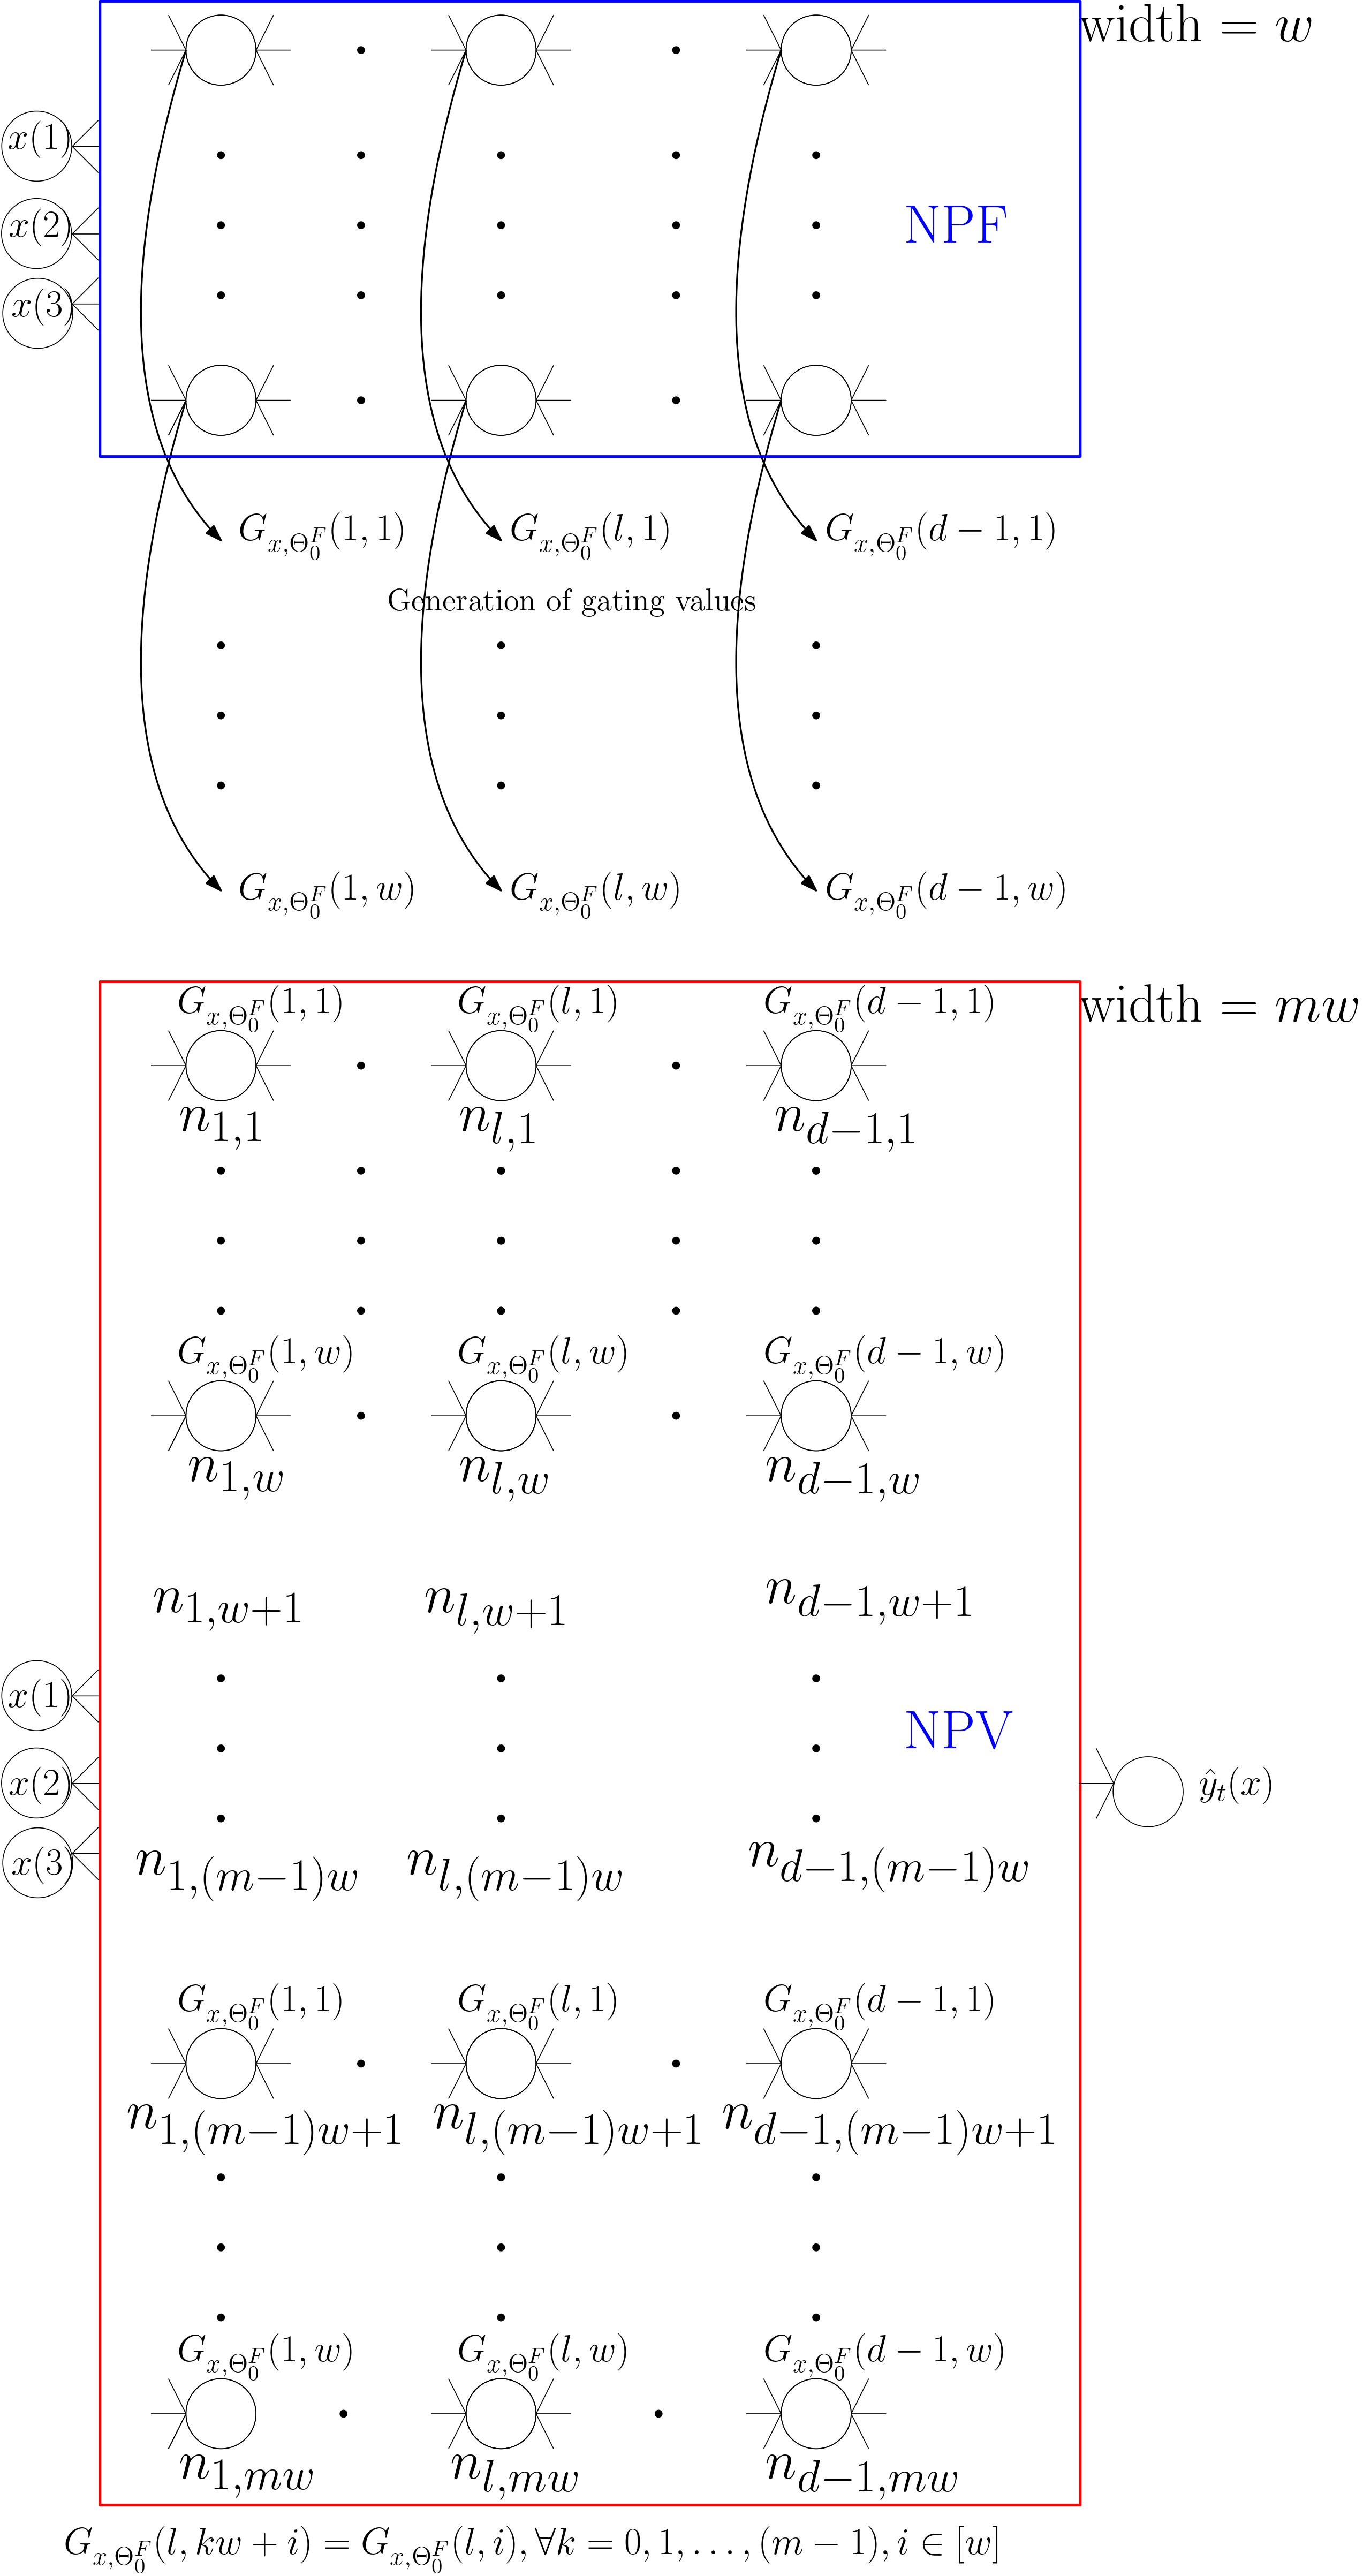
\includegraphics[scale=0.1]{figs/dgn-infty-flipped.png}
%}
\caption{DGN${}^{(m)}$ where the value network is of width $mw$ and depth $d$. The gates are derived by padding the gating values obtained from the feature network `$m$' times, i.e., $ G_{x,t}(l,kw+i)=G_{x,t}(l,i),\forall k=0,1,\ldots,m-1, i\in[w]$.}
\label{fig:dgnpad}
\end{figure}

\begin{table}
\centering
\begin{tabular}{|l|l|l|}\hline
Layer& Feature Network (NPF)& Value Network (NPV)\\
Input & $z^{\text{F}}_{x,t}(0)=x$ &$z^{\text{V}}_{x,t}(0)=x$ \\
Activation & $q^{\text{F}}_{x,t}(l)={\Tg_t(l)}^\top z^{\text{F}}_{x,t}(l-1)$& $q^{\text{V}}_{x,t}(l)={\Tv_t(l)}^\top z^{\text{V}}_{x,t}(l-1)$\\
Hidden &$z^{\text{F}}_{x,t}(l)=\chi^{\text{F}}\left(q^{\text{F}}_{x,t}(l)\right)$& $z^{\text{V}}_{x,t}(l)=q^{\text{V}}_{x,t}(l)\odot G_{x,t}(l)$ \\
Output & None &$\hat{y}_t(x)={\Tv(d)}^\top z^{\text{V}}_{x,t}(d-1)$\\\hline
\multicolumn{3}{|l|}{Gating Values:\quad$ G_{x,t}(l)= \gamma_{r}\left(q^{\text{F}}_{x,t}(l)\right)\quad$or $G_{x,t}(l)= \gamma_{sr}\left(q^{\text{F}}_{x,t}(l)\right)$}\\\hline
\end{tabular}
\caption{Deep Gated Network with padding. Here the gating values are padded, i.e., $ G_{x,t}(l,kw+i)=G_{x,t}(l,i),\forall k=0,1,\ldots,m-1, i\in[w]$. }
\label{tb:dgnpad}
\end{table}

\textbf{Remark:}  DGN${}^{(m)}$ has a total of $P^{(m)}=(mw)^{(d-1)}d_{in}$ paths. Thus, the NPF and NPV are quantities in $\R^{P^{(m)}}$. In what follows, we denote the NPF matrix of DGN${}^{(m)}$ by $\Phi^{(m)}_{\Tg_0}\in\R^{P^{(m)}\times n}$, and use $H^{(m)}_{\text{FNPF}}=(\Phi^{(m)}_{\Tg_0})^\top \Phi^{(m)}_{\Tg_0}$. 

Before we proceed to state the version of \Cref{th:main} for DGN${}^{(m)}$, we will look at an equivalent definition for $\Lambda_{\Theta}$ (see \Cref{def:lambda}).
\begin{definition}\label{def:equilambda}
For input examples $s, s'\in[n]$ define 

$1.$ $\tau_{\Theta}(s,s',l)\stackrel{def}=\sum_{i=1}^w G_{x_s,\Theta}(l,i)G_{x_{s'},\Theta}(l,i)$ be the number of activations that are ``on'' for both inputs $s,s'\in[n]$ in layer $l\in[d-1]$.

$2.$ $\Lambda_{\Theta}(s,s')\stackrel{def}=\Pi_{l=1}^{d-1}\tau_{\Theta}(s,s',l)$.
\end{definition}



\begin{corollary}[Corollary to \Cref{th:main}] Under \Cref{assmp:main} with $\sigma$ replaced by $\sigma_{(m)}=\sigma/\sqrt{m}$, as $m\ra\infty$, $K_{\Theta^{\text{DGN}^{(m)}}_0}\ra K^{(d)}_{\text{FNPF}} = d\cdot \sigma_{(m)}^{2(d-1)} H^{(m)}_{\text{FNPF}}= d\cdot \sigma^{2(d-1)} H_{\text{FNPF}}$.
\end{corollary}
\begin{proof}
Let $\Lambda^{(m)}_{\text{FNPF}}$ and $\tau^{(m)}_{\text{FNPF}}$ be quantities associated with DGN${}^{(m)}$. We know that  $H^{(m)}_{\text{FNFP}}=\Sigma\odot\Lambda^{(m)}_{\text{FNPF}}$. Dropping the subscript FNPF to avoid notational clutter, we have
\begin{align*}
\left(\sigma/\sqrt{m}\right)^{2(d-1)}\Lambda^{(m)}(s,s')&=\sigma^{2(d-1)}\frac{1}{m^{(d-1)}}\Pi_{l=1}^{d-1}\tau^{(m)}(s,s',l)\\
&=\sigma^{2(d-1)}\frac{1}{m^{(d-1)}}\Pi_{l=1}^{d-1}\left(m \tau(s,s',l)\right)\\
&=\sigma^{2(d-1)}\frac{1}{m^{(d-1)}}m^{(d-1)}\Pi_{l=1}^{d-1} \tau(s,s',l)\\
&=\sigma^{2(d-1)}\Pi_{l=1}^{d-1} \tau(s,s',l)\\
&=\sigma^{2(d-1)}\Lambda(s,s')
\end{align*}
\end{proof}


\section{Proofs of technical results}
Proof of \Cref{prop:basic}
\begin{proof}
We know that $e_t=(e_t(s),s\in[n])\in\R^n$, and $e_t(s)=\hat{y}_{\Theta_t}(x_s)-y(s)$. Now
\begin{align} 
L_{\Theta_t}&=\frac{1}2\sum_{s'=1}^n(\hat{y}_{\Theta_t}-y)^2\nn\\
&=\frac{1}2\sum_{s'=1}^n e_t^2\nn\\
\nabla_{\Theta} L_{\Theta_t}&= \sum_{s'=1}^n\nabla_{\Theta} \hat{y}_{\Theta_t}(x_{s'})e_t(s')\nn\\
\label{eq:above1} \nabla_{\Theta} L_{\Theta_t}&= \sum_{s'=1}^n \psi_{x_{s'},\Theta_t}e_t(s')
\end{align}
For gradient descent, $\dot{\Theta}_t=-\nabla_{\Theta} L_{\Theta_t}$, from \eqref{eq:above1} it follows that 
\begin{align}
\dot{\Theta}_t=-\sum_{s'=1}^n \psi_{x_{s'},\Theta_t}e_t(s')
\end{align}
Now $\dot{e}_t=\dot{\hat{y}}_{\Theta_t}$, and expanding $\dot{\hat{y}}_{\Theta_t}(x_s)$ for some $s\in[n]$, we have:
\begin{align}
\dot{\hat{y}}_{\Theta_t}(x_s)&=\frac{d \hat{y}_{\Theta_t}(x_s)}{d t}\nn\\
&=\sum_{\theta\in\Theta}\frac{d \hat{y}_{\Theta_t}(x_s)}{d \theta}\frac{d \theta_t}{dt},\,\text{by expressing this summation as a dot product we obtain} \nn\\
\dot{\hat{y}}_{\Theta_t}(x_s)&=\ip{\psi_{x_s,\Theta_t},\dot{\Theta}_t}
\end{align}
We now use that fact that $\Theta_t$ is updated by gradient descent
\begin{align}
\dot{\hat{y}}_{\Theta_t}(x_s)&=-\ip{\psi_{x_s,\Theta_t},\sum_{s'=1}^n \psi_{x_{s'},\Theta_t}e_t(s')}\nn\\
&=-\sum_{s'=1}^n K_{\Theta_t}(s,s')e_t(s')
\end{align}
The proof is complete by recalling that $\hat{y}_{\Theta_t}=(\hat{y}_{\Theta_t}(x_s),s\in[n])$, and $\dot{e}_t=\dot{\hat{y}}_{\Theta_t}$.
\end{proof}


Proof of \Cref{prop:zero}
\begin{proof}
Let $x\in\R^{d_{in}}$ be the input to the DNN and $\hat{y}_{\Theta}(x)$ be its output. The output can be written in terms of the final hidden layer output 
\begin{align}
\hat{y}_{\Theta}(x)&={\Theta(d)}^\top z_{x,\Theta}(d-1)\nn\\
&=\sum_{j_{d-1}=1}^w\Theta(d, j_{d-1},1)  z_{x,\Theta}(d-1,j_{d-1})\nn\\
\label{lastlayer}&=\sum_{j_{d-1}=1}^w\Theta(d, j_{d-1},1)  G_{x\Theta}(d-1,j_{d-1}) q_{x,\Theta}(d-1,j_{d-1})
\end{align}
Now $q_{x,\Theta}(d-1,j_{d-1})$ for a fixed $j_{d-1}$ can again be expanded as
\begin{align}
q_{x,\Theta}(d-1,j_{d-1})&= \sum_{j_{d-2}=1}^w \Theta(d, j_{d-2}, j_{d-1}) z_{x,\Theta}(d-2,j_{d-2})\nn\\
\label{onebefore}&=\sum_{j_{d-2}=1}^w \Theta(d-1, j_{d-2}, j_{d-1}) G_{x,\Theta}(d-2,j_{d-2})q_{x,\Theta}(d-2,j_{d-2})
\end{align}
Now plugging in \eqref{onebefore} in the expression in \eqref{lastlayer}, we have
\begin{align}
\hat{y}_{\Theta}(x)&=\sum_{j_{d-1}=1}^w\Theta(d, j_{d-1},1)  G_{x\Theta}(d-1,j_{d-1}) \left(\sum_{j_{d-2}=1}^w \Theta(d-1, j_{d-2}, j_{d-1}) G_{x,\Theta}(d-2,j_{d-2})q_{x,\Theta}(d-2,j_{d-2})\right)\nn\\
&=\sum_{j_{d-1}, j_{d-2}\in[w]} G_{x,\Theta}(d-1,j_{d-1}) G_{x,\Theta}(d-2,j_{d-2}) \Theta(d, j_{d-1},1) \Theta(d-1, j_{d-2}, j_{d-1}) q_{x,\Theta}(d-2,j_{d-2})\nn\\
\end{align}
By expanding $q$'s for all the previous layers till the input layer we have
\begin{align}
\sum_{j_{d}=1, j_{d-1},\ldots,j_{1}\in[w], j\in[d_{in}]} x(j) \Pi_{l=1}^{d-1}G_{x,\Theta}(l,j_{l}) \Pi_{l=1}^{d}\Theta(l, j_{l-1}, j_{l}) \nn
\end{align}
\end{proof}

Proof of \Cref{lm:npk}
\begin{proof}
\begin{align}
\ip{\phi_{x_s,\Theta},\phi_{x_{s'},\Theta}}&=\sum_{p\in[P]}x_s(\I_0(p))x_{s'}(\I_0(p))A_{\Theta}(x_s,p)A_{\Theta}(x_{s'},p)\nn\\
&=\sum_{i=1}^{d_{in}}x_s(i)x_{s'}(i)\Lambda_{\Theta}(s,s')\nn\\
&=\ip{x_s,x_{s'}}\cdot\Lambda_{\Theta}(s,s')
\end{align}
\end{proof}

Proof of \Cref{prop:ntknew}
\begin{proof}
Let $\Psi_{\Theta}=(\psi_{x_s,\Theta},s\in[n])\in\R^{d_{net}\times n}$ be the NTF matrix, then the NTK matrix is given by $K_{\Theta_t}=\Psi^\top_{\Theta_t}\Psi_{\Theta_t}$. Note that, $\hat{y}_{\Theta}(x_s)=\ip{\phi_{x_s,\Theta},v_{\Theta}}=\ip{v_{\Theta},\phi_{x_s,\Theta}}=v^\top_{\Theta}\phi_{x_s,\Theta}$. Now $\psi_{x_{s},\Theta}=\nabla_{\Theta} v_{\Theta}\phi_{x_s,\Theta}$, and hence $\Psi=\nabla_{\Theta} v_{\Theta}\Phi_{\Theta}$. Hence, $K_{\Theta_t}=\Psi^\top_{\Theta_t}\Psi_{\Theta_t}=\Phi^\top_{\Theta}(\nabla_{\Theta} v_{\Theta})^\top (\nabla_{\Theta} v_{\Theta})\Phi_{\Theta}=\Phi^\top_{\Theta}\V_{\Theta}\Phi_{\Theta}$.
\end{proof}

Proof of \Cref{prop:dnnhard}

\begin{proof}
Follows in a similar manner as the proof of \Cref{prop:basic}.
\end{proof}

Proof of {\Cref{prop:condition}}
\begin{proof}
$\rho_{\min}(K_{\Theta})=\underset{\norm{x}_2=1}{\underset{x\in \R^n}\min}x^\top K_{\Theta} x$. Let $x'\in\R^n$ such that $\norm{x'}_2=1$ and $\rho_{\min}(K_{\Theta})={x'}^\top K_{\Theta} x'$. Now, let $y'=\Phi x'$. Then we have, $\rho_{\min}(K_{\Theta})={y'}^\top \V_{\Theta}y'$. Hence $\rho_{\min}(K_{\Theta})\leq \norm{y'}^2_2 \rho_{\max}(\V_{\Theta})$. Now, $\norm{y'}^2_2={x'}^\top \Phi^\top_{\Theta}\Phi_{\Theta}x'\leq \rho_{min}(H_{\Theta})$.
\end{proof}


Proof of \Cref{prop:dgn}

\begin{proof}
Follows in a similar manner as proof of \Cref{prop:basic}.
\end{proof}


\begin{lemma}\label{lm:dot}
Let $\varphi_{p,\Theta}$ be as in \Cref{def:npvgrad}, under Assumption~\ref{assmp:main}, for paths $p,p_1,p_2\in \P, p_1\neq p_2$, at initialisation we have (i) $\E{\ip{\varphi_{p_1,\Tv_0}, \varphi_{p_2,\Tv_0}}}= 0$, (ii) ${\ip{\varphi_{p,\Tv_0}, \varphi_{p,\Tv_0}}}= d\sigma^{2(d-1)}$.
\end{lemma}

\begin{proof}
\begin{align*}
\ip{\varphi_{p_1,\Tv_0}, \varphi_{p_2,\Tv_0}}= \sum_{\tv\in \Tv} \partial_{\tv}v_{\Tv_0}(p_1) \partial_{\tv}v_{\Tv_0}(p_2)
\end{align*}
Let $p\rsa(\cdot)$ denote the fact that path $p$ passes through $(\cdot)$, and let $p\bcancel\rsa(\cdot)$ denote the fact that path $p$ does not pass through $\bcancel\rsa$. Let $\tv\in\Tv$ be any weight such that $p\rsa \tv$, and w.l.o.g let $\tv$ belong to layer $l'\in[d]$. If either $p_1\bcancel{\rsa}\tv$ or $p_2\bcancel{\rsa}\tv$, then it follows that $\partial_{\tv} v_{\Tv_0}(p_1) \partial_{\tv} v_{\Tv_0}(p_2)=0$. In the case when $p_1,p_2\rsa\tv$, we have
\begin{align*}
&\E{\partial_{\tv}v_{\Tv_0}(p_1)\partial_{\tv}v_{\Tv_0}(p_2)}\\
&=\E{\underset{l\neq l'}{\underset{l=1}{\overset{d}{\Pi}}} \Bigg(\Tv_0(l, \I_{l-1}(p_1),\I_{l} (p_1))\Tv_0(l,\I_{l-1} (p_2),\I_{l}(p_2)) \Bigg)}\\
&=\underset{l\neq l'}{\underset{l=1}{\overset{d}{\Pi}}}\E{\Tv_0(l,\I_{l-1}(p_1),\I_{l}(p_1))\Tv_0(l,\I_{l-1}(p_2),\I_{l}(p_2))}
\end{align*}
where the $\E{\cdot}$ moved inside the product because at initialisation the weights (of different layers) are independent of each other.
Since $p_1\neq p_2$, in one of the layers $\tilde{l}\in[d-1],\tilde{l}\neq l'$ they do not pass through the same weight, i.e., $\Tv_0(\tilde{l},\I_{\tilde{l}-1}(p_1),\I_{\tilde{l}}(p_1))$ and $\Tv_0(\tilde{l},\I_{\tilde{l}-1}(p_2),\I_{\tilde{l}}(p_2))$ are distinct weights. Using this fact
\begin{align*}
&\E{\partial_{\tv}v_{\Tv_0}(p_1)\partial_{\tv}v_{\Tv_0}(p_2)}\\
&=\underset{l\neq l',\tilde{l}}{\underset{l=1}{\overset{d}{\Pi}}}\E{\Tv_0(l, \I_{l-1}(p_1),\I_l(p_1))\Tv_0(l,\I_{l-1}(p_2),\I_{l}(p_2))}\\
&=\E{\Tv_0(\tilde{l},\I_{\tilde{l}-1} (p_1),\I_{\tilde{l}}(p_1))}\E{\Tv_0(\tilde{l},\I_{\tilde{l}-1 }(p_2),\I_{\tilde{l}}(p_2))}\\
&=0
\end{align*}

The proof of (ii) is complete by noting that $\sum_{\tv\in\Tv} \partial_{\tv}v_{\Tv_0}(p) \partial_{\tv}v_{\Tv_0}(p)$ has $d$ non-zero terms for a single path $p$ and at initialisation we have 
\begin{align*}
&\partial_{\tv}v_{\Tv_0}(p) \partial_{\tv}v_{\Tv_0}(p) \\
&={\underset{l\neq l'}{\underset{l=1}{\overset{d}{\Pi}}} {\Tv_0}^2(l,\I_{l-1}(p),\I_{l}(p))}\\
&=\sigma^{2(d-1)}
\end{align*}
\end{proof}

\textbf{Detailed version of \Cref{th:main} with proof.}
\begin{theorem}\label{th:mainrefined}
Under \Cref{assmp:main}, and $\frac{4d}{w^2}<1$ it follows that
 \begin{align*}
\E{K_{\Tdgn_0}}&=d\cdot\sigma^{2(d-1)} H_{\text{FNPF}}\\
Var\left[K_{\Tdgn_0}(s,s')\right]&\leq O\left(d^2_{in}\sigma^{4(d-1)}\max\{d^2w^{2(d-2)+1}, d^3w^{2(d-2)}\}\right)
\end{align*}
\end{theorem}

\begin{proof}
We have 
\begin{align*}
\E{K_{\Tdgn_0}}&=\E{\Phi^\top_{\text{FNPF}} \V_{\Tv_0} \Phi_{\text{FNPF}}}\\
&=\E{\Phi^\top_{\text{FNPF}} (\nabla_{\Tv}v_{\Tv_0})^\top (\nabla_{\Tv}v_{\Tv_0}) \Phi_{\text{FNPF}}}\\
&=\Phi^\top_{\text{FNPF}} \E{(\nabla_{\Tv}v_{\Tv_0})^\top (\nabla_{\Tv}v_{\Tv_0})}\Phi_{\text{FNPF}}\\
&\stackrel{(a)}=d\cdot\sigma^{2(d-1)} \Phi^\top_{\text{FNPF}}\Phi_{\text{FNPF}}\\
&=d\cdot\sigma^{2(d-1)} H_{\text{FNPF}}
\end{align*}
where, $(a)$ follows from \Cref{lm:dot}.

We now turn to the variance calculation. The idea is that we expand  $Var\left[K_0(s,s')\right]=\E{K_0(s,s')^2} -\E{K_0(s,s')}^2$ and identify the terms which cancel due to subtraction and then bound the rest of the terms.

\textbf{Notation:} In what follows, we let $K_0$ to denote $K_{\Tdgn_0}$ and drop superscript V from $\Tv_0$, and subscript $\Tv_0$ from $v_{\Tv_0}$. Further, we assume that the weights can be enumerated as $\theta(1),\ldots, \theta(d_{net})$. We also denote $p\rsa (\cdot)$ to denote the fact that path $p$ passes through $(\cdot)$ and $p\bcancel{\rsa}(\cdot)$ to denote the fact that path $p$ does not pass through $(\cdot)$. We use a shortcut notation $A(s,p)$ instead of $A(x_s,p)$. In what follows, we let $x\in\R^{d_{in}\times n}$ to be the data matrix.

 Let $\theta(m),m\in[d_{net}]$ belong to layer $l'(m)$, then 
\begin{align}\label{eq:kexpect} 
&\E{K_0(s,s')}\nn\\
&=\sum_{m=1}^{d_{net}}\E{\left(\sum_{p_1 \in[P]}x(\I_0(p_1),s)A_0(s,p_1)\frac{\partial v_0(p_1)}{\partial \theta(m)}\right)\left(\sum_{p_2\in[P]}x(\I_0(p_2),s)A_0(s',p_2)\frac{\partial v_0(p_2)}{\partial \theta(m)}\right)}\nn\\
&=\sum_{m=1}^{d_{net}}\E{\sum_{p_1,p_2\in[P]}x(\I_0(p_1),s)A_0(s,p_1)\frac{\partial v_0(p_1)}{\partial \theta(m)}x(\I_0(p_2),s')A_0(s',p_2)\frac{\partial v_0(p_2)}{\partial \theta(m)}}\nn\\
&\stackrel{(a)}=\sum_{m=1}^{d_{net}}\underset{p_1,p_2\rsa\theta(m)}{\sum_{p_1,p_2\in[P]}}x(\I_0(p_1),s)A_0(s,p_1)x(\I_0(p_2),s')A_0(s',p_2) \mathbb{E}\Bigg[\underset{l\neq l'(m)}{\underset{l=1}{\overset{d-1}{\Pi}}} \Tb_0(l,\I_{l-1}(p_1),\I_{l}(p_1)) \nn\\&\Tb_0(l,\I_{l-1}(p_2),\I_{l}(p_2))\Bigg]\nn\\
&\stackrel{(b)}=\sum_{m=1}^{d_{net}}\underset{p_1,p_2\rsa\theta(m)}{\sum_{p_1,p_2\in[P]}}x(\I_0(p_1),s)A_0(s,p_1)x(\I_0(p_2),s')A_0(s',p_2) \underset{l\neq l'(m)}{\underset{l=1}{\overset{d-1}{\Pi}}} \mathbb{E}\Bigg[ \Tb_0(l,\I_{l-1}(p_1),\I_{l}(p_1))\nn\\
& \Tb_0(l,\I_{l-1}(p_2),\I_{l}(p_2))\Bigg]
\end{align}
where $(a)$ follows from the fact that for $p\bcancel{\rsa}\theta(m)$, $\frac{\partial v_0(p)}{\partial \theta(m)}=0$, and $(b)$ follows from the fact that at initialisation the layer weights are independent of each other. Note that the right hand side of \eqref{eq:kexpect} only terms with $p_1=p_2$ will survive the expectation.

In the following expression in \eqref{eq:kexpectsquare}, note that only terms of the form $p_1=p_2$ and $p_3=p_4$ are non-zero.

\begin{align*}
&\E{K_0(s,s')}^2=\\
&\Bigg(\sum_{m=1}^{d_{net}}\underset{p_1,p_2\rsa\theta(m)}{\sum_{p_1,p_2\in[P]}}x(\I_0(p_1),s)A_0(s,p_1)x(\I_0(p_2),s')A_0(s',p_2) \underset{l\neq l'(m)}{\underset{l=1}{\overset{d-1}{\Pi}}} \mathbb{E}\Big[\Tb_0(l,\I_{l-1}(p_1),\I_{l}(p_1)) &\\ 
&\Tb_0(l,\I_{l-1}(p_2),\I_{l}(p_2))\Big]\Bigg)\times\\
&\Bigg(\sum_{m'=1}^{d_{net}}\underset{p_3,p_4\rsa\theta(m')}{\sum_{p_3,p_4\in[P]}}x(\I_0(p_3),s)A_0(s,p_3)x(\I_0(p_4),s')A_0(s',p_4) \underset{l\neq l'(m')}{\underset{l=1}{\overset{d-1}{\Pi}}} \mathbb{E}\Big[\Tb_0(l,\I_{l-1}(p_3),\I_{l}(p_3)) &\\
&\Tb_0(l,\I_{l-1}(p_4),\I_{l}(p_4))\Big]\Bigg)\\
\end{align*}
\begin{align}\label{eq:kexpectsquare}
&\E{K_0(s,s')}^2=\nn\\
&\sum_{m,m'=1}^{d_{net}}\underset{p_3,p_4\rsa\theta(m')}{\underset{p_1,p_2\rsa\theta(m)}{\sum_{p_1,p_2,p_3,p_4\in[P]}}}\Bigg[\bigg(x(\I_0(p_1),s)A_0(s,p_1)x(\I_0(p_2),s')A_0(s',p_2)x(\I_0(p_3),s)\nn\\ 
&A_0(s,p_3)x(\I_0(p_4),s')A_0(s',p_4)\bigg)\times \bigg( \underset{l\neq l'(m)} {\underset{l\neq l'(m')}{\underset{l=1}{\overset{d-1}{\Pi}}}} \E{\Tb_0(l,\I_{l-1}(p_1),\I_{l}(p_1)) \Tb_0(l,\I_{l-1}(p_2),\I_{l}(p_2))}\nn\\
&\E{\Tb_0(l,\I_{l-1}(p_3),\I_{l}(p_3)) \Tb_0(l,\I_{l-1}(p_4),\I_{l}(p_4))} \bigg)\times\nn\\
&\bigg( \E{\Tb_0(l,\I_{l'(m')-1}(p_1),\I_{l'(m')}(p_1)) \Tb_0(l,\I_{l'(m')-1}(p_2),\I_{l'(m')}(p_2))}\bigg)\times\nn\\
&\bigg(\E{\Tb_0(l,\I_{l'(m)-1}(p_3),\I_{l'(m)}(p_3)) \Tb_0(l,\I_{l'(m)-1}(p_4),\I_{l'(m)}(p_4))} \bigg)\Bigg]
\end{align}
In the expression in \eqref{eq:ksquareexpect}, paths $p_1,p_2,p_3,p_4$ do not have constraints, and can be distinct.
\begin{align}\label{eq:ksquareexpect}
&\E{K^2_0(s,s')}=\nn\\
&\sum_{m,m'=1}^{d_{net}}\underset{p_3,p_4\rsa\theta(m')}{\underset{p_1,p_2\rsa\theta(m)}{\sum_{p_1,p_2,p_3,p_4\in[P]}}}\Bigg[\bigg(x(\I_0(p_1),s)A_0(s,p_1)x(\I_0(p_2),s')A_0(s',p_2)x(\I_0(p_3),s)\nn\\&
A_0(s,p_3)x(\I_0(p_4),s')A_0(s',p_4)\bigg)\times\bigg( \underset{l\neq l'(m)} {\underset{l\neq l'(m')}{\underset{l=1}{\overset{d-1}{\Pi}}}} \mathbb{E}[\Tb_0(l,\I_{l-1}(p_1),\I_{l}(p_1)) \Tb_0(l,\I_{l-1}(p_2),\I_{l}(p_2))\nn\\&
\Tb_0(l,\I_{l-1}(p_3),\I_{l}(p_3)) \Tb_0(l,\I_{l-1}(p_4),\I_{l}(p_4))] \bigg)\times\nn\\
&\bigg( \E{\Tb_0(l,\I_{l'(m')-1}(p_1),\I_{l'(m')}(p_1)) \Tb_0(l,\I_{l'(m')-1}(p_2),\I_{l'(m')}(p_2))}\bigg)\times\nn\\
&\bigg(\E{\Tb_0(l,\I_{l'(m)-1}(p_3),\I_{l'(m)}(p_3)) \Tb_0(l,\I_{l'(m)-1}(p_4),\I_{l'(m)}(p_4))} \bigg)\Bigg]
\end{align}

We now state the following facts/observations.

$\bullet$ \emph{Fact 1:} Any term that survives the expectation (i.e., does not become $0$) and participates in \eqref{eq:ksquareexpect} is of the form $\sigma^{4(d-1)}\big(x(\I_0(p_1),s)A_0(s,p_1)x(\I_0(p_2),s')A_0(s',p_2)x(\I_0(p_3),s)A_0(s,p_3)x(\I_0(p_4),s')A_0(s',p_4)\big)$, where $p_1,p_2,p_3,p_4$ are free variables. Any term that survives the expectation (i.e., does not become $0$) and participates in participates in \eqref{eq:kexpectsquare} is of the form $\sigma^{4(d-1)}\big(x(\I_0(p_1),s)A_0(s,p_1)x(\I_0(p_2),s')A_0(s',p_2)x(\I_0(p_3),s)A_0(s,p_3)x(\I_0(p_4),s')A_0(s',p_4)\big)$, where $p_1=p_2,p_3=p_4$.

$\bullet$ \emph{Fact 2:} The number of paths through a particular weight $\theta(m)$ in one of the middle layers is $d_{in}w^{d-3}$. The number of paths through a particular weight $\theta(m)$ in the first layer is $w^{d-2}$ . The number of paths through a particular weight $\theta(m)$ in the last layer is $d_{in}w^{d-2}$ .


$\bullet$ \emph{Fact 3:} Let $\P'$ be an arbitrary set of paths constrained to pass through some set of weights. Let $\P''$ be the set of paths obtained by adding an additional constraint that the paths also should pass through a particular weight say $\theta(m)$. Now, if $\theta(m)$ belongs to :

$1.$ a middle layer, then $|\P''|=\frac{|\P'|}{w^2}$.

$2.$ the first layer, then $|\P''|=\frac{|\P'|}{d_{in}w}$.

$3.$  the last layer, then $|\P''|=\frac{|\P'|}{w}$.

$\bullet$ \emph{Fact 4:} For any $p_1,p_2,p_3,p_4$ combination that survives the expectation in \eqref{eq:ksquareexpect} can be written as 

\begin{align*}
&\bigg(x(\I_0(p_1),s)A_0(s,p_1)x(\I_0(p_2),s')A_0(s',p_2)x(\I_0(p_3),s)\\
&A_0(s,p_3)x(\I_0(p_4),s')A_0(s',p_4)\bigg)\times\\
&\bigg( \underset{l\neq l'(m)} {\underset{l\neq l'(m')}{\underset{l=1}{\overset{d-1}{\Pi}}}} \mathbb{E}[\Tb_0(l,\I_{l-1}(p_1),\I_{l}(p_1)) \Tb_0(l,\I_{l-1}(p_2),\I_{l}(p_2))\nn\\
&\Tb_0(l,\I_{l-1}(p_3),\I_{l}(p_3)) \Tb_0(l,\I_{l-1}(p_4),\I_{l}(p_4))] \bigg)\times\nn\\
&\bigg( \E{\Tb_0(l,\I_{l'(m')-1}(p_1),\I_{l'(m')}(p_1)) \Tb_0(l,\I_{l'(m')-1}(p_2),\I_{l'(m')}(p_2))}\bigg)\times\nn\\
&\bigg(\E{\Tb_0(l,\I_{l'(m)-1}(p_3),\I_{l'(m)}(p_3)) \Tb_0(l,\I_{l'(m)-1}(p_4),\I_{l'(m)}(p_4))} \bigg)\nn\\
%&=\\
%&\bigg( \underset{l\neq l'(m)} {\underset{l\neq l'(m')}{\underset{l=1}{\overset{d-1}{\Pi}}}} \Tb^2_0(l,\I_{l-1}(\rho_a),\I_{l}(\rho_a)) \Tb^2_0(l,\I_{l-1}(\rho_b),\I_{l}(\rho_b)) \bigg)\times \bigg( \Tb^2_0(l,\I_{l'(m')-1}(\rho_a),\I_{l'(m')}(\rho_a))\bigg)\nn\\
%&\times \bigg({\Tb^2_0(l,\I_{l'(m)-1}(\rho_b),\I_{l'(m)}(\rho_b))} \bigg),
\end{align*}

where $\rho_a\rsa \theta(m)$ and $\rho_b\rsa \theta(m')$ are what we call as \emph{base} (case) paths. 


$\bullet$ \emph{Fact 5:} For any given base paths $\rho_a$ and $\rho_b$ there could be multiple assignments possible for $p_1,p_2,p_3,p_4$.

$\bullet$ \emph{Fact 6:}  Terms in \eqref{eq:ksquareexpect}, wherein, the base case is generated as $p_1=p_2=\rho_a$ and $p_3=p_4=\rho_b$ (or $p_1=p_2=\rho_b$ and $p_3=p_4=\rho_a$), get cancelled with the corresponding terms in \eqref{eq:kexpectsquare}.

$\bullet$ \emph{Fact 7:}  When the bases paths $\rho_a$ and $\rho_b$ do not intersect (i.e., do not pass through the same weight in any one of the layers), the only possible assignment is $p_1=p_2=\rho_a$ and $p_3=p_4=\rho_b$ (or $p_1=p_2=\rho_b$ and $p_3=p_4=\rho_a$), and such terms are common in \eqref{eq:ksquareexpect} and \eqref{eq:kexpectsquare}, and hence do not show up in the variance term.


$\bullet$ \emph{Fact 7:} Let base paths $\rho_a$ and $\rho_b$ intersect/cross at layer $l_1, \ldots, l_k, k \in [d-1]$, and let $\rho_a=(\rho_a(1),\ldots,\rho_a(k+1))$ where $\rho_a(1)$ is a sub-path string from layer $1$ to $l_1$, and $\rho_a(2)$ is the sub-path string from layer $l_1+1$ to $l_2$ and so on, and $\rho_a(k+1)$ is the sub-path string from layer $l_k+1$ to the output node. Then the set of paths that can occur in $\E{K_0(s,s')^2}$ are of the form:
\begin{enumerate}
\item $p_1=p_2=\rho_a, p_3=p_4=\rho_b$ (or $p_1=p_2=\rho_b, p_3=p_4=\rho_a$) which get cancelled in the $\E{K_0(s,s')}^2$ term.
\item $p_1=\rho_a$, $p_3=\rho_b$, $p_2=(\rho_b(1),\rho_a(2),\rho_a(3),\ldots,\rho_a(k+1))$, $p_4=(\rho_a(1),\rho_b(2),\rho_b(3),\ldots,\rho_b(k+1))$, which are obtained by \emph{splicing} the base paths in various combinations. Note that for such spliced paths $p_1\neq p_2$ and $p_3\neq p_4$ and hence do not occur in the expression for $\E{K_0(s,s')}^2$ in \eqref{eq:kexpectsquare}.
\end{enumerate}


$\bullet$ \emph{Fact 8:} For $k$ crossings of the base paths there are $4^{k+1}$ splicings possible, and those many terms are extra in the $\E{K_0(s,s')^2}$ expression in \eqref{eq:ksquareexpect}, when compared to the $\E{K_0(s,s')}^2$ expression in \eqref{eq:kexpectsquare}. 

\textbf{Upper Bound:} We now enumerate various possible crossings of the base paths, and calculate an upper bound for the magnitude of the contribution of `spliced' terms to the variance term using the \emph{Fact 1} to \emph{Fact 8}. In short, we find an upper bound for the those terms that do not get cancelled in the variance calculation. Further, without loss of generality we drop $x(\I_0(p))$ and $A(\cdot,\cdot)$ terms in this upper calculation.

\textbf{Case $1$:} $k=1$ crossing, in either first or last layer. There are $d_{in}w$ weights in the first layer and $w$ weights in the last layer. The number of base path combinations passing through the first layer is $w^{d-2}\times w^{d-2}$. The number of base path combinations passing through the last layer is ($d_{in}w^{d-2})\times (d_{in}w^{d-2})$.  For each of these cases, $m,m'$ could take $O(d^2)$ possible values. And the multiplication of the weights themselves contribute to $\sigma^{4(d-1)}$.  Splicing of these base paths could be done in $4^2$ ways. Putting them together we have
\begin{align*}
&\sigma^{4(d-1)}\times(w)\times (d^2_{in} \times w^{d-2}\times w^{d-2})\times d^2\times 4^2\\
&+\sigma^{4(d-1)}\times (d_{in}w) \times(w^{d-2}\times w^{d-2}) \times d^2\times  4^2\\
&\leq 32d^2_{in}\sigma^{4(d-1)}d^2 w^{2(d-2)+1}
\end{align*}

\textbf{Case $2$:} $k=1$ crossing, in one of the middle layers. There are $w^2(d-2)$ weights in the middle layers. The number of base path combinations  that pass through a given weight in the middle layers is $(d_{in}w^{d-3})\times(d_{in} w^{d-3})$. For each of these cases, $m,m'$ could take $O(d^2)$ possible values. And the multiplication of the weights themselves contribute to $\sigma^{4(d-1)}$. Splicing of these base paths could be done in $4^2$ ways. Putting them together we have
\begin{align*}
\sigma^{4(d-1)} \times w^2(d-2)\times (d^2_{in}\times w^{d-3}\times w^{d-3})\times d^2 \times 4^2\leq 16d^2_{in}\sigma^{4(d-1)} d^3 w^{2(d-3)}
\end{align*}

\textbf{Case $3$:} $k=2$ crossings, one in the first layer and other in the last layer. %This case can be covered using Case $1$ and then further restricting that the base paths should also in the other layer. 
So, we have
%\begin{align*}
%32d^2_{in}\sigma^{4(d-1)}d^2 w^{2(d-2)+1} \times \underbrace{w}_{\text{possible weights in other layer}} \times \underbrace{w^{-1}\times w^{-1}}_{\text{reduction in paths due to additional restriction}} \times 4 = (32d^2_{in}\sigma^{4(d-1)}d^2 w^{2(d-2)+1})\times (4w^{-1}),
%\end{align*}

\begin{align*}
\sigma^{4(d-1)} (d_{in}w \times w) \times (w^{(d-3)} \times w^{(d-3)}) d^2 \times 4^3 \leq (32d^2_{in}\sigma^{4(d-1)}d^2 w^{2(d-2)+1})\times (4w^{-1}),
\end{align*}


%\begin{align*}
%32d^2_{in}\sigma^{4(d-1)}d^2 w^{2(d-2)+1} \times {w} \times {w^{-1}\times w^{-1}}\times 4 = (32d^2_{in}\sigma^{4(d-1)}d^2 w^{2(d-2)+1})\times (4w^{-1}),
%\end{align*}

%where the $4$ is for the $4$ extra possible ways of splicing the base paths.

\textbf{Case $4$:} $k=2$ crossings, first one in the first layer or the last layer, and the second one in the middle layer. This can be obtained by looking at the Case $1$ and then adding the further restriction that the base paths should cross each other in the middle layer. 
\begin{align*}
&32d^2_{in}\sigma^{4(d-1)}d^2 w^{2(d-2)+1}\times w^2(d-2) \times w^{-2}\times w^{-2}\times 4\\
&\leq (32d^2_{in}\sigma^{4(d-1)}d^2 w^{2(d-2)+1} )\times (4dw^{-2}) 
\end{align*}

\textbf{Case $5$:} $k=2$ crossings, in the middle layer. This can be obtained by taking Case $2$ and then adding the further restriction that the base paths should cross each other in the middle layer. 
\begin{align*}
16d^2_{in}\sigma^{4(d-1)} d^3 w^{2(d-3)}\times w^2(d-2) \times w^{-2}\times w^{-2}\times 4\leq (16d^2_{in}\sigma^{4(d-1)} d^3 w^{2(d-3)}) \times (4dw^{-2})
\end{align*}


\textbf{Case $6$:} $k=3$ crossings, first one in the first layer or the last layer, and the other two in the middle layers. This can be obtained by considering Case $4$ and then adding the further restriction that the base paths should cross each other in the middle layer. 
\begin{align*}
(32d^2_{in}\sigma^{4(d-1)}d^2 w^{2(d-2)+1} )\times (4dw^{-2}) \times (4dw^{-2}) 
\end{align*}

\textbf{Case $7$:} $k=3$ crossings, first two in the first and last layers and the third one in the middle layers. This can be obtained by considering Case $3$ and then adding the further restriction that the base paths should cross each other in the middle layer. 

\begin{align*}
(32d^2_{in}\sigma^{4(d-1)}d^2 w^{2(d-2)+1})\times (4w^{-1})\times (4dw^{-2}) 
\end{align*}

\textbf{Case $8$:} $k=3$ crossings, in the middle layer. This can be obtained by considering Case $5$ and then adding the further restriction that the base paths should cross each other in the middle layer. 
\begin{align*}
 (16d^2_{in}\sigma^{4(d-1)} d^3 w^{2(d-3)}) \times (4dw^{-2})\times (4dw^{-2}) 
\end{align*}


The cases can be extended in a similar way, increasing the number of crossings.  Now, assuming $\frac{4d}{w^2}<1$, the bounds in the various terms can be lumped together as below:

$\bullet$ We can add the bounds for Case $1$, Case $4$, Case $6$ and other cases obtained by adding more crossings (one at a time) in the middle layer to Case $6$. This gives rise to a term which is upper bounded by (for some constant $C>0$): 
\begin{align*}
C d^2_{in}\sigma^{4(d-1)}d^2w^{2(d-2)+1}\left(\frac{1}{1-4dw^{-2}}\right)
\end{align*}

$\bullet$ We can add the bounds for Case $3$, Case $7$ and other cases obtained by adding more crossings (one at a time) in the middle layer to Case $6$. This gives rise to a term which is upper bounded by 
\begin{align*}
C d^2_{in}\sigma^{4(d-1)}d^3w^{2(d-2)} \left(\frac{1}{1-4dw^{-2}}\right)
\end{align*}



$\bullet$ We can add the bounds for Case $2$, Case $5$, Case $8$ and other cases obtained by adding more crossings (one at a time) in the middle layer to Case $6$. This gives rise to a term which is upper bounded by 
\begin{align*}
C d^2_{in}\sigma^{4(d-1)}d^2w^{2(d-2)} \left(\frac{1}{1-4dw^{-2}}\right)
\end{align*}

Putting together we have the variance to be bounded by 
\begin{align*}
Cd^2_{in}\sigma^{4(d-1)}\max\{d^2w^{2(d-2)+1}, d^3w^{2(d-2)}\},
\end{align*}
for some constant $C>0$.
\end{proof}




\section{DGN as a Lookup Table: Applying \Cref{th:main} to a pure memorisation task}

In this section, we modify the DGN in \Cref{fig:dgn} into a memorisation network to solve a pure memorisation task. The objective of constructing the memorisation network is to understand the roles of depth and width in \Cref{th:main} in a simplified setting. In this setting, we show increasing depth till a point helps in training and increasing depth beyond it hurts training. 

\begin{definition}[Memorisation Network/Task]
Given a set of values $(y_s)_{s=1}^n\in  \R$, a memorisation network (with weights $\Theta\inrdnet$) accepts $s\in[n]$ as its input and produces $\hat{y}_{\Theta}(s)\approx y_s$ as its output. The loss of the memorisation network is defined as $L_{\Theta}=\frac{1}{2}\sum_{s=1}^n (\hat{y}_{\Theta}(s)-y_s)^2$.
\end{definition}
\FloatBarrier
\begin{table}[h]
\centering
\begin{tabular}{| l |  l  |}\hline
Layer&  Memorisation Network\\\hline
Input  &$z_{t}(0)=1$ \\
Activation & $q_{s,t}(l)={\Theta_t(l)}^\top z_{s,t}(l-1)$\\
Hidden & $z_{s,t}(l)=q_{s,t}(l)\odot G_{s,t}(l)$ \\
Output & $\hat{y}_t(s)={\Theta(d)}^\top z_{s,t}(d-1)$\\\hline
\end{tabular}
\caption{ Memorisation Network. The input is fixed and is equal to $1$. All the internal variables depend on the index $s$ and the parameter $\Theta_t$. The gating values $G$s are external and independent variables.}
\label{tb:dgnmemo}
\end{table}

\textbf{Fixed Random Gating:} The memorisation network is described in \Cref{tb:dgnmemo}. In a memorisation network, the gates are \emph{fixed and random}, i.e., for each index $s\in[n]$, the gating values $G_{s,0}(l,i),\forall l\in[d-1], i\in[w] $ are sampled from $Ber(\mu), \mu\in(0,1)$ taking values in $\{0,1\}$,  and kept fixed throughout training, i.e., $G_{s,t}(\cdot,\cdot)=G_{s,0}(\cdot,\cdot)\,\forall\,t\geq 0$. The input to the memorisation network is fixed as $1$, and since the gating is fixed and random there is a separate random sub-network to memorise each target $y_s\in\R$. The memorisation network can be used to memorise the targets  $(y_s)_{s=1}^n$ by training it using gradient descent by minimising the squared loss $L_{\Theta}$. In what follows, we let $K_0$ and $H_0$ to be the NTK and NPK of the memorisation network at initialisation.


\textbf{Performance of Memorisation Network:} From \Cref{prop:basic} we know that as $w\ra\infty$, the training error dynamics of the memorisation network follows:
\begin{align}
\dot{e}_t=-K_{0} e_t,
\end{align}
i.e., the spectral properties of $K_0$ (or $H_0$) dictates the rate of convergence of the training error to $0$. In the case of the memorisation network with fixed and random gates, we can calculate $\E{K_0}$ explicitly. 

\textbf{Spectrum of $H_0$:}The input Gram matrix $\Sigma$ is a $n\times n$ matrix with all entries equal to $1$ and its rank is equal to 1, and hence $H_0=\Lambda_0$. We can now calculate the properties of $\Lambda_0$. It is easy to check that $\mathbb{E}_{\mu}\left[\Lambda_0(s,s)\right]=(\mu w)^{(d-1)},\forall s\in[n]$ and $\mathbb{E}_{\mu}\left[\Lambda_0(s,s')\right]=(\mu^2 w)^{(d-1)},\forall s,s'\in[n]$.  For $\sigma=\sqrt{\frac{1}{\mu w}}$, and $\mathbb{E}_{\mu}\left[K_0(s,s)/d\right]=1$, and $\mathbb{E}_{\mu}\left[K_0(s,s')/d\right]=\mu^{(d-1)}$. 
\begin{figure}
\centering
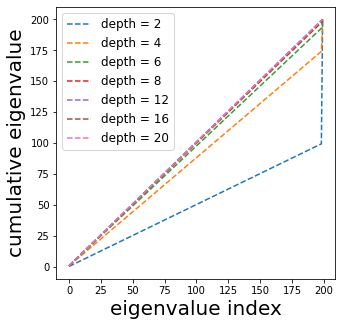
\includegraphics[scale=0.3]{figs/dgn-fra-ecdf-ideal-small.png}
\caption{Ideal spectrum of $\E{K_0}/d$ for a memorisation network for $n=200$.}
\label{fig:ideal-spectrum}
\end{figure}


\textbf{Why increasing depth till a point helps ?} 
We have:
%\comment{
\begin{align}\label{eq:mat}
\frac{\E{K_0}}{d}=\left[\begin{matrix}
1 &\mu^{d-1} &\ldots &\mu^{d-1} &\ldots\\ 
\ldots &1 &\ldots &\mu^{d-1} &\ldots\\ 
\ldots &\mu^{d-1} &\ldots &1 &\ldots \\
\ldots &\mu^{d-1} &\ldots &\mu^{d-1} &1\\ 
\end{matrix}\right]
\end{align}
%}
i.e., all the diagonal entries are $1$ and non-diagonal entries are $\mu^{d-1}$. Now, let $\rho_i\geq 0,i \in [n]$ be the eigenvalues of $\frac{\E{K_0}}{d}$, and let $\rho_{\max}$ and $\rho_{\min}$ be the largest and smallest eigenvalues.  One can easily show that $\rho_{\max}=1+(n-1)\mu^{d-1}$ and corresponds to the eigenvector with all entries as $1$, and $\rho_{\min}=(1-\mu^{d-1})$ repeats $(n-1)$ times,  which corresponds to eigenvectors given by $[0, 0, \ldots, \underbrace{1, -1}_{\text{$i$ and $i+1$}}, 0,0,\ldots, 0]^\top \in \R^n$ for $i=1,\ldots,n-1$. Note that as $d\ra\infty$, $\rho_{\max},\rho_{\min}\ra 1$.

\textbf{Why increasing depth beyond a point hurts?} 
In \Cref{th:mainrefined}, note that for a fixed width $w$, as the depth increases the variance of the entries $K_0(s,s')$ deviates from its expected value $\E{K_0(s,s')}$. Thus the structure of the Gram matrix degrades from \eqref{eq:mat}, leading to smaller eigenvalues.
\FloatBarrier
\begin{figure}[h]
\resizebox{\textwidth}{!}{
\begin{tabular}{cccc}
%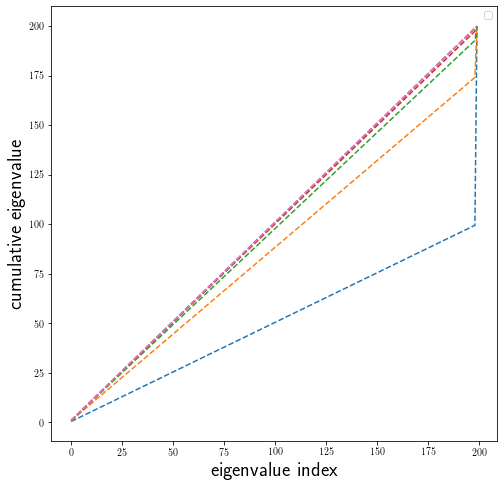
\includegraphics[scale=0.4]{figs/dgn-fra-ecdf-ideal.png}
%&
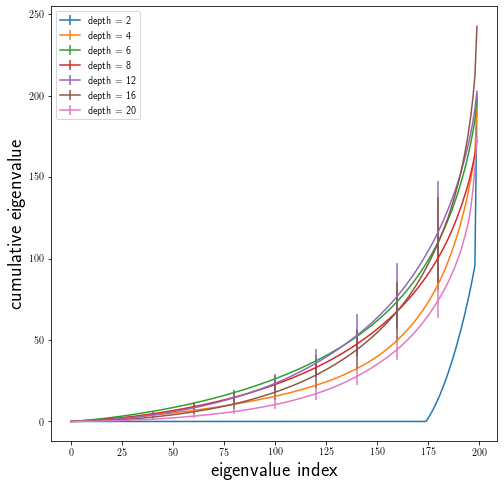
\includegraphics[scale=0.5]{figs/dgn-fra-ecdfbyd-w25.png}
&
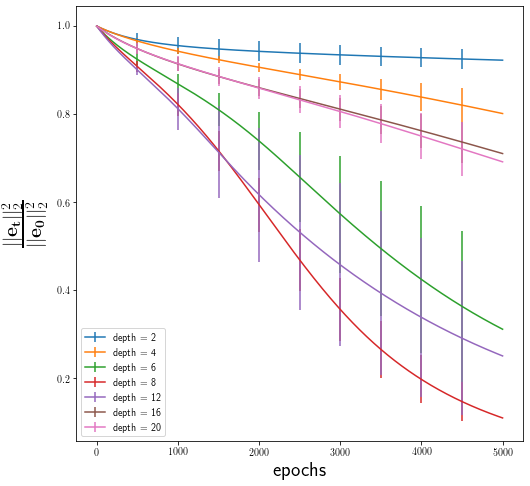
\includegraphics[scale=0.5]{figs/dgn-fra-conv-w25.png}
&
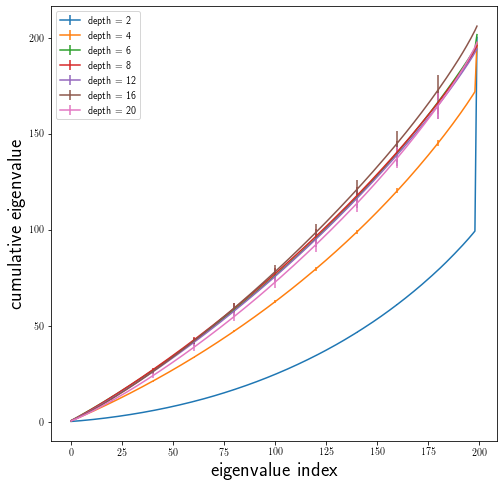
\includegraphics[scale=0.5]{figs/dgn-fra-ecdfbyd-w500.png}
&
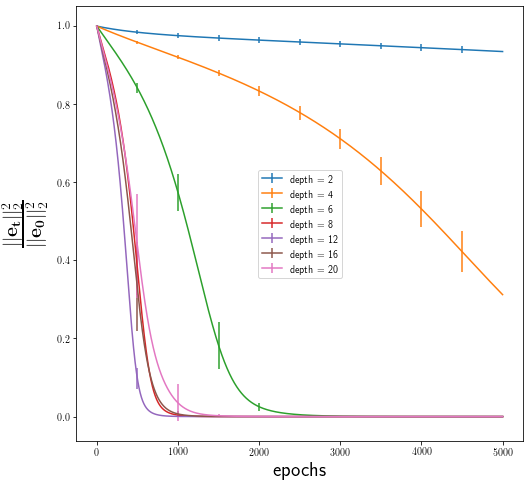
\includegraphics[scale=0.5]{figs/dgn-fra-conv-w500.png}
\end{tabular}
}
\caption{Shows the plots for the memorisation network with $\mu=\frac{1}{2}$ and $\sigma=\sqrt{\frac{2}{w}}$. The number of points to be memorised is $n=200$. The left most plot shows the e.c.d.f for $w=25$ and the second plot from the left shows the error dynamics during training for $w=25$. The second plot from the right shows the e.c.d.f for $w=500$ and the right most plot shows the error dynamics during training for $w=500$. All plots are averaged over $10$ runs.}
\label{fig:dgn-frg-gram-ecdf}
\end{figure}

\subsection{Experiment}
We set $n=200$, and $y_s\sim\text{Uniform}[-1,1]$. We look at the cumulative eigenvalue (e.c.d.f) obtained by first sorting the eigenvalues in ascending order then looking at their cumulative sum. The ideal behaviour (\Cref{fig:ideal-spectrum}) as predicted from theory is that for indices $k\in[n-1]$, the e.c.d.f should increase at a linear rate, i.e., the cumulative sum of the first $k$ indices is equal to $k(1-\mu^{d-1})$, and the difference between the last two indices is $1+(n-1)\mu^{d-1}$. In \Cref{fig:dgn-frg-gram-ecdf}, we plot the actual e.c.d.f for various depths $d=2,4,6,8,12,16,20$ and $w=25,500$ (first and third plots from the left in \Cref{fig:dgn-frg-gram-ecdf}). 

\textbf{Roles of depth and width:} In order to compare how the rate of convergence varies with the depth, we set the step-size $\alpha=\frac{0.1}{\rho_{\max}}$, $w=100$. We use the vanilla SGD-optimiser. Note the$ \frac{1}{\rho_{\max}}$ in the stepsize, ensures that the uniformity of maximum eigenvalue across all the instances, and the convergence should be limited by the smaller eigenvalues. We also look at the convergence rate of the ratio $\frac{\norm{e_t}^2_2}{\norm{e_0}^2_2}$. We notice that for $w=25$, increasing depth till $d=8$ improves the convergence, however increasing beyond $d=8$ worsens the convergence rate. For $w=500$, increasing the depth till $d=12$ improves convergence, and $d=16,20$ are worse than $d=12$.  %This matches with the depth phenomena observed in practical DNNs and also matches our theory.


\end{appendix}

\end{document}
